%% ============================================================================
%%  Formalized foundations for the discrete dynamic programming theory
%%  of the normalized p-Laplacian, in Lean 4.
%%
%%  Technical companion to the article "A formally verified convergence
%%  theorem for the tug-of-war scheme of the normalized p-Laplacian".
%%  It documents the development at tag v1.3, layer by layer.
%%
%%  \LEANREF{..} gives the Lean declaration name backing a statement.
%% ============================================================================

\documentclass[11pt,reqno]{amsart}

\usepackage{amsmath,amssymb,amsthm,mathtools}
\newcommand{\fint}{\mathop{\mathrlap{\,\rule[0.62ex]{0.62em}{0.5pt}}\int}}
\usepackage[margin=1.1in]{geometry}
\usepackage{fancyvrb}
\usepackage{xcolor}
\usepackage{iftex}
\usepackage{booktabs}
\usepackage{longtable}
\usepackage{tikz}
\usetikzlibrary{arrows.meta,positioning,fit}

\definecolor{leanbg}{RGB}{247,247,250}

\ifPDFTeX
  \usepackage[T1]{fontenc}
  \usepackage[utf8]{inputenc}
  \newcommand{\leanfont}{\ttfamily}
  \DeclareUnicodeCharacter{00B7}{\ensuremath{\cdot}}
  \DeclareUnicodeCharacter{00D7}{\ensuremath{\times}}
  \DeclareUnicodeCharacter{0393}{\ensuremath{\Gamma}}
  \DeclareUnicodeCharacter{039B}{\ensuremath{\Lambda}}
  \DeclareUnicodeCharacter{03A9}{\ensuremath{\Omega}}
  \DeclareUnicodeCharacter{03B1}{\ensuremath{\alpha}}
  \DeclareUnicodeCharacter{03B2}{\ensuremath{\beta}}
  \DeclareUnicodeCharacter{03B4}{\ensuremath{\delta}}
  \DeclareUnicodeCharacter{03B5}{\ensuremath{\varepsilon}}
  \DeclareUnicodeCharacter{03B8}{\ensuremath{\theta}}
  \DeclareUnicodeCharacter{03BB}{\ensuremath{\lambda}}
  \DeclareUnicodeCharacter{03C3}{\ensuremath{\sigma}}
  \DeclareUnicodeCharacter{03C6}{\ensuremath{\varphi}}
  \DeclareUnicodeCharacter{03C8}{\ensuremath{\psi}}
  \DeclareUnicodeCharacter{2080}{\ensuremath{{}_0}}
  \DeclareUnicodeCharacter{2081}{\ensuremath{{}_1}}
  \DeclareUnicodeCharacter{2082}{\ensuremath{{}_2}}
  \DeclareUnicodeCharacter{2098}{\ensuremath{{}_m}}
  \DeclareUnicodeCharacter{2099}{\ensuremath{{}_n}}
  \DeclareUnicodeCharacter{2115}{\ensuremath{\mathbb{N}}}
  \DeclareUnicodeCharacter{211D}{\ensuremath{\mathbb{R}}}
  \DeclareUnicodeCharacter{2124}{\ensuremath{\mathbb{Z}}}
  \DeclareUnicodeCharacter{2190}{\ensuremath{\leftarrow}}
  \DeclareUnicodeCharacter{2192}{\ensuremath{\rightarrow}}
  \DeclareUnicodeCharacter{21A6}{\ensuremath{\mapsto}}
  \DeclareUnicodeCharacter{21D2}{\ensuremath{\Rightarrow}}
  \DeclareUnicodeCharacter{2200}{\ensuremath{\forall}}
  \DeclareUnicodeCharacter{2203}{\ensuremath{\exists}}
  \DeclareUnicodeCharacter{2208}{\ensuremath{\in}}
  \DeclareUnicodeCharacter{2209}{\ensuremath{\notin}}
  \DeclareUnicodeCharacter{2211}{\ensuremath{\sum}}
  \DeclareUnicodeCharacter{2218}{\ensuremath{\circ}}
  \DeclareUnicodeCharacter{2227}{\ensuremath{\wedge}}
  \DeclareUnicodeCharacter{2228}{\ensuremath{\vee}}
  \DeclareUnicodeCharacter{2229}{\ensuremath{\cap}}
  \DeclareUnicodeCharacter{222A}{\ensuremath{\cup}}
  \DeclareUnicodeCharacter{222B}{\ensuremath{\int}}
  \DeclareUnicodeCharacter{2260}{\ensuremath{\neq}}
  \DeclareUnicodeCharacter{2264}{\ensuremath{\leq}}
  \DeclareUnicodeCharacter{2265}{\ensuremath{\geq}}
  \DeclareUnicodeCharacter{2286}{\ensuremath{\subseteq}}
  \DeclareUnicodeCharacter{27E8}{\ensuremath{\langle}}
  \DeclareUnicodeCharacter{27E9}{\ensuremath{\rangle}}
  \DeclareUnicodeCharacter{2A05}{\ensuremath{\sqcap}}
  \DeclareUnicodeCharacter{2A06}{\ensuremath{\bigsqcup}}
  \DeclareUnicodeCharacter{2A0D}{\ensuremath{\fint}}
  \DeclareUnicodeCharacter{221E}{\ensuremath{\infty}}
  \DeclareUnicodeCharacter{221A}{\ensuremath{\sqrt{}}}
  \DeclareUnicodeCharacter{2016}{\ensuremath{\|}}
  \DeclareUnicodeCharacter{02E2}{\ensuremath{^{\mathrm{s}}}}
  \DeclareUnicodeCharacter{2A2F}{\ensuremath{\times}}
\else
  % ------------------------------------------------------------------------
  % XeLaTeX / LuaLaTeX branch.
  %
  % THE SUPPORTED ENGINE FOR THIS DOCUMENT IS pdfLaTeX. Use it unless you have
  % a specific reason not to; on Overleaf, Menu -> Compiler -> pdfLaTeX.
  %
  % This branch requires the Latin Modern Math OpenType font to be installed
  % and findable. If it is not, \setmathfont fails silently and every math
  % alphabet is left without a font, producing errors of the form
  %   "Math alphabet identifier \mathrm is undefined in math version normal"
  % or
  %   "\textfont 6 is undefined".
  % Neither is recoverable from within the document. Check availability with
  %   fc-list | grep -i "latin modern math"
  % and switch to pdfLaTeX if it is absent.
  % ------------------------------------------------------------------------
  \usepackage{fontspec}
  \usepackage{unicode-math}
  \setmathfont{Latin Modern Math}
  % unicode-math does not assign a font to the \mathrm range by itself, and
  % \sup, \inf and \operatorname are internally \mathop{\mathrm{...}}.
  % Without the next line every one of them errors with
  %   "Math alphabet identifier \mathrm is undefined in math version normal".
  \setmathfont{Latin Modern Roman}[range={\mathrm,\mathup},
    Scale=MatchUppercase]
  \setmathfont{Latin Modern Roman}[range={\mathit},
    Scale=MatchUppercase, ItalicFont={Latin Modern Roman Italic}]
  \setmathfont{Latin Modern Roman}[range={\mathbf},
    Scale=MatchUppercase, BoldFont={Latin Modern Roman Bold}]
  \newfontfamily\leanfont{DejaVu Sans Mono}[Scale=0.82]
\fi

\fvset{
  formatcom=\leanfont,
  frame=single,
  framerule=0pt,
  rulecolor=\color{leanbg},
  xleftmargin=4pt,
  fontsize=\small
}
\DefineVerbatimEnvironment{lean}{Verbatim}{}

\usepackage[colorlinks=true,linkcolor=blue,citecolor=blue,urlcolor=blue]{hyperref}

\setlength{\emergencystretch}{3em}

\newcommand{\TODOcol}{red}
\long\def\TODO#1{{\color{red}\textbf{[TODO: }#1\textbf{]}}}
\long\def\CHECK#1{{\color{orange}\textbf{[CHECK: }#1\textbf{]}}}
\newcommand{\LEANREF}[1]{\texttt{\small\def\_{\textunderscore\allowbreak}#1}}
\newcommand{\normPLapOfName}{\LEANREF{normPLapOf}}
\newcommand{\viscF}{\ensuremath{\mathcal{F}}}

\newcommand{\R}{\mathbb{R}}
\newcommand{\N}{\mathbb{N}}
\newcommand{\eps}{\varepsilon}
\newcommand{\dlap}{\Delta}
\newcommand{\pnlap}{\Delta_p^{N}}
\newcommand{\inflap}{\Delta_\infty^{N}}
\newcommand{\Op}{T_\eps}
\newcommand{\avgint}{\fint}
\DeclarePairedDelimiter{\abs}{\lvert}{\rvert}
\DeclarePairedDelimiter{\norm}{\lVert}{\rVert}
\newcommand{\usc}{\operatorname{usc}}
\newcommand{\lsc}{\operatorname{lsc}}

\theoremstyle{plain}
\newtheorem{theorem}{Theorem}[section]
\newtheorem{proposition}[theorem]{Proposition}
\newtheorem{lemma}[theorem]{Lemma}
\newtheorem{corollary}[theorem]{Corollary}
\theoremstyle{definition}
\newtheorem{definition}[theorem]{Definition}
\newtheorem{remark}[theorem]{Remark}
\newtheorem{assumption}[theorem]{Assumption}
\newtheorem{finding}[theorem]{Finding}

% ============================================================================
\begin{document}

\title[Formalized convergence for the normalized $p$-Laplacian:
       technical companion]
      {A formalized convergence theory\\
       for the dynamic programming scheme\\
       of the normalized $p$-Laplacian:\\
       technical companion}

\author{Juan J. Manfredi}
\address{Department of Mathematics, University of Pittsburgh,
  Pittsburgh, PA 15260, USA}
\email{manfredi@pitt.edu}

\author{Behrooz Moosavi}
\address{Department of Mathematics, University of Pittsburgh,
  Pittsburgh, PA 15260, USA}
\email{behroozmoosavi@pitt.edu}

\date{\today}

\subjclass[2020]{68V20, 35J92, 49L20, 35D40}
\keywords{normalized $p$-Laplacian, dynamic programming, $p$-harmonious
  functions, viscosity solutions, tug-of-war, Lean, formalized mathematics,
  measurability}

\begin{abstract}
This document is the technical companion to the article \emph{A formally
verified convergence theorem for the tug-of-war scheme of the normalized
$p$-Laplacian}. It describes, layer by layer, a Lean~4 formalization of the
convergence of $p$-harmonious functions, the solutions of the dynamic
programming principle of tug-of-war with noise, to the viscosity solution of
the Dirichlet problem for the normalized $p$-Laplacian, $2 \le p < \infty$.
Layer~1 is the discrete theory: the step operator, the measurability that makes
its admissible class invariant, existence by iteration, and the discrete
comparison principle. Layer~2 is the viscosity framework. Layer~3 is the
asymptotic expansion of the scheme, with an explicit error rate. Layer~4 proves
the viscosity property of the half-relaxed limits, Alexandrov's theorem,
Jensen's lemma, the comparison principle and uniqueness for the homogeneous
equation, the
boundary behaviour under an exterior sphere condition, uniform convergence, and
existence and uniqueness for the $\eps$-problem with exterior data, so that the
main theorem holds unconditionally.
Every statement is given with the name of the Lean declaration that proves it.
We also record fifty-one findings in which formalization corrected or
constrained the intended development, and describe the architecture of the 223
files and
the techniques that mattered. The development contains no unproved statements,
and its main theorem depends only on Lean's standard axioms.
\end{abstract}

\maketitle

% ============================================================================
\section{Introduction}\label{sec:intro}

\subsection*{About this document}
This is the technical companion to the article \cite{MMart}. The article
states the main theorem, explains the strategy of the proof and selects the
most instructive findings; this document supplies the detail. Each layer of
the development has its own section (\S\S\ref{sec:layer1}--\ref{sec:conv}),
in which definitions and theorems are stated as they are formalized, with the
Lean declaration that proves each one shown in typewriter type. The findings
are collected in \S\ref{sec:findings}, the file-by-file architecture in
\S\ref{sec:arch}, and notes on formalization technique in
\S\ref{sec:notes}. The sections can be read independently, and a reader
interested in a single result can go directly to its section.

\subsection{The equation}

For $1 < p < \infty$ the \emph{normalized}, or \emph{game-theoretic},
$p$-Laplacian is
\begin{equation}\label{eq:pnlap}
  \pnlap u \;=\; \dlap u + (p-2)\,\inflap u,
  \qquad
  \inflap u \;=\; \Bigl\langle D^2 u \,\tfrac{\nabla u}{\abs{\nabla u}},\,
                             \tfrac{\nabla u}{\abs{\nabla u}} \Bigr\rangle,
\end{equation}
defined where $\nabla u \ne 0$. Unlike the variational $p$-Laplacian, the
operator \eqref{eq:pnlap} is $1$-homogeneous and not in divergence form, so it
has no weak formulation and the natural notion of solution is the viscosity
one.

\subsection{The dynamic programming route}

Peres, Schramm, Sheffield and Wilson introduced tug-of-war, a two-player
zero-sum game in which a fair coin decides at each turn which player moves a
token a distance at most $\eps$, and identified the infinity Laplacian as the
generator of its continuum limit \cite{PSSW09}. Mixing the tug with a random
step, as in the tug-of-war with noise of Peres and Sheffield \cite{PS08},
reaches the normalized $p$-Laplacian for finite $p$; Manfredi, Parviainen and
Rossi made this precise through the asymptotic mean value characterization of
$p$-harmonic functions \cite{MPR10} and through $p$-harmonious functions, the
solutions of the associated discrete problem \cite{MPR12}.

The structural point for this development is that the value of the $\eps$-step game
satisfies a dynamic programming principle, and both the discrete
well-posedness theory and the convergence theory can be developed on that
principle alone, without constructing the game: the analytic existence and
uniqueness proof of Luiro, Parviainen and Saksman \cite{LPS14} needs no
probability, and the convergence argument of Barles and Souganidis \cite{BS91}
needs only monotonicity, stability and consistency of the scheme. We follow
both routes, and exclude the probabilistic layer by design.

\subsection{What is formalized}\label{ssec:scope}

For $2 \le p < \infty$ and a bounded domain $\Omega \subseteq \R^d$:

\emph{Layer 1, the discrete theory.}
\begin{itemize}
  \item the $\eps$-step operator, with monotonicity, translation equivariance
        and nonexpansiveness (Theorem~\ref{thm:one});
  \item Borel measurability of the extreme values over open balls
        (Theorem~\ref{thm:meas}), and invariance of the admissible class
        (Theorem~\ref{thm:invariance});
  \item the boundary strip and the $\eps$-Dirichlet problem, with the
        containment making the problem closed (Lemma~\ref{lem:closed});
  \item the Perron iteration, and the estimate of \cite{LPS14} for its uniform
        convergence (Theorems~\ref{thm:iteration}--\ref{thm:existence});
        existence itself is assembled in \S\ref{ssec:dirichlet};
  \item \textbf{the comparison principle}, from which uniqueness follows
        (Theorems~\ref{thm:comparison}, \ref{thm:comparisonfinal}).
\end{itemize}

\emph{Layer 2, the viscosity framework.}
\begin{itemize}
  \item the operator in generator form, with $1$-homogeneity in the Hessian,
        invariance under positive scaling of the gradient, and degenerate
        ellipticity (Theorem~\ref{thm:elliptic});
  \item the sub- and supersolution predicates, with the singular set
        $\{\nabla u = 0\}$ treated through closed-form envelopes
        (\S\ref{ssec:visc});
  \item the second-order necessary condition, in one variable
        (Theorem~\ref{thm:so1}) and in several (Theorem~\ref{thm:somulti});
  \item \textbf{consistency with classical solutions}
        (Theorem~\ref{thm:consistency});
  \item \textbf{stability} under restriction, addition of a constant,
        addition of a smooth function, and finite maxima
        (\S\ref{ssec:stability}).
\end{itemize}

\emph{Layer 3, the asymptotic expansion.}
\begin{itemize}
  \item the second-order Taylor expansion with an explicit cubic bound
        (Theorem~\ref{thm:taylor}), which Mathlib does not provide in several
        variables;
  \item the moment library at arbitrary radius, and the average of a quadratic
        form over a ball (Theorem~\ref{thm:quadavg});
  \item \textbf{the average expansion} (Theorem~\ref{thm:avgexp});
  \item the localization of the maximizer (Theorem~\ref{thm:localize}) and the
        \textbf{extreme-value expansion} (Theorem~\ref{thm:extexp});
  \item the singular case, where the envelopes of Layer 2 reappear
        (Theorem~\ref{thm:singexp});
  \item \textbf{the expansion of the step operator}
        (Theorem~\ref{thm:opexp});
  \item the error at an explicit rate: the Taylor error cubic in the
        increment (Theorem~\ref{thm:cubicrate}), the average error cubic
        (Theorem~\ref{thm:avgrate}), and the weighted total bounded by its
        halves (Theorem~\ref{thm:opbounded}).
\end{itemize}

\emph{Auxiliary results, of independent interest.} Monotonicity of the Bochner
set average (Theorem~\ref{thm:avgmono}); all moments of order $\le 2$ of
Lebesgue measure on a ball (Theorem~\ref{thm:moments}).

\emph{Layer 4, convergence.}
\begin{itemize}
  \item the half-relaxed limits, finite, ordered and semicontinuous
        (Theorem~\ref{thm:relaxed});
  \item the comparison through the operator with a local and approximate
        contact (Theorem~\ref{thm:approxcmp});
  \item near-maximizers and their convergence to the point of contact
        (Theorems~\ref{thm:nearsup}, \ref{thm:nearfreq});
  \item the expansion uniform in the base point (Theorem~\ref{thm:expunif});
  \item the four core inequalities at strict extrema, regular and singular
        (Theorems~\ref{thm:regsub}, \ref{thm:regsup}, \ref{thm:singsub},
        \ref{thm:singsup});
  \item the reductions to general test functions at local extrema
        (Theorems~\ref{thm:regularize}, \ref{thm:c2reduce});
  \item \textbf{the relaxed limits are viscosity sub- and supersolutions}
        (Theorem~\ref{thm:main4});
  \item the comparison principle for strict subsolutions, with the theorem
        of sums (Theorems~\ref{thm:strictcomp}, \ref{thm:sums});
  \item \textbf{Alexandrov's theorem} and \textbf{Jensen's lemma}
        (Theorems~\ref{thm:alexandrov}, \ref{thm:jensen});
  \item the strong maximum and minimum principles (Theorem~\ref{thm:smp});
  \item \textbf{the comparison principle} for the homogeneous equation, and
        uniqueness of viscosity solutions
        (Theorems~\ref{thm:viscomp}, \ref{thm:viscunique});
  \item the discrete comparison against a strict supersolution, the boundary
        barrier, and \textbf{the boundary estimate} under an exterior sphere
        condition (Theorems~\ref{thm:disccomp}, \ref{thm:barrier},
        \ref{thm:bdry});
  \item \textbf{convergence}: $u_\eps$ converges uniformly on
        $\overline\Omega$ to the viscosity solution (Theorem~\ref{thm:main});
  \item \textbf{existence and uniqueness} for the $\eps$-problem with
        exterior data, and the main theorem in unconditional form
        (Theorems~\ref{thm:dirunif}, \ref{thm:existsph},
        \ref{thm:existsconv}, \ref{thm:discunique}).
\end{itemize}

\emph{Not formalized.} The stability of an infinite family of subsolutions
(\S\ref{sec:future}), and the stability estimate of \cite[Theorem~2.2]{LPS14}
for solutions with different boundary data; uniqueness for equal data is
formalized (Theorem~\ref{thm:discunique}).

\emph{Not attempted.} The game itself. No strategy spaces, path-space
measures, stopping times or optional stopping arguments appear. The dynamic
programming principle is the \emph{definition} of the discrete problem, not a
consequence of play; Finding~\ref{find:mpr} records the price of that decision.

\subsection{Contributions}

\begin{enumerate}
  \item A complete machine-checked well-posedness theory for the discrete
        problem, following the analytic route of \cite{LPS14}. (2791 lines.)
  \item A viscosity framework for the limiting equation: operator, predicates,
        consistency and stability. (1122 lines.)
  \item The asymptotic expansion of the step operator, with both halves, the
        singular case, the error at an explicit rate, and the $C^2$ estimate.
        (4300 lines.)
  \item The viscosity property of the half-relaxed limits, against the
        layer-two predicates with $C^2$ test functions, at regular and
        singular points. (About 8000 lines, of which roughly a third belong to
        a first route that was superseded.)
  \item The comparison principle for the homogeneous limit equation: the
        theorem of sums, the strong maximum principle, and a translation
        argument that supplies the strictness the equation lacks at critical
        points. (About 9000 lines, including the next two items.)
  \item Alexandrov's theorem, through the proximal map, with neither the
        Hahn--Banach theorem nor integration; absent from Mathlib.
        (About 1250 lines.)
  \item Jensen's lemma, with neither mollification nor the area formula;
        absent from Mathlib. (About 530 lines.)
  \item The boundary behaviour of the relaxed limits under an exterior sphere
        condition, the convergence theorem, and existence and uniqueness for
        the $\eps$-problem with exterior data. (About 2200 lines.)
  \item \LEANREF{setAverage\_mono}, absent from Mathlib: monotonicity of
        $\avgint$ over a general set. Mathlib has the $\mathrm{ENNReal}$-valued
        lower average and circle averages, but not this. (95 lines.)
  \item The second-order necessary condition at an interior local extremum,
        absent from Mathlib, which has Fermat's theorem but nothing of second
        order. (141 lines.)
  \item The complete second-moment tensor of a Euclidean ball, with the
        single-coordinate reflection \LEANREF{flipCoordEquiv} as reusable
        infrastructure. (398 lines.)
  \item Fifty-one findings (\S\ref{sec:findings}), two of them structural,
        one constraining how second-order analysis can be formalized at all,
        one on the difference between a proof that typechecks and a statement
        that says something, one on the informal proof's shape not being the
        right shape for the formal one, one --- correcting our own earlier
        claim --- on a library's missing theorem being evidence about the
        library rather than about what the proof needs, and two on the
        convergence argument that we believe are of interest beyond
        formalization: the singular inequality needs no singularity, and the
        reduction to smooth test functions needs only the quadratic form. Nine
        more come from the comparison principle and the boundary: among them,
        that translation supplies the strictness missing at critical points,
        that a single point of Jensen's set suffices, and that no barrier need
        ever be differentiated.
\end{enumerate}

\subsection{Code availability}

The development is written in Lean~4 \cite{dMU21} on top of the Mathlib
library \cite{Mathlib20}. Lean toolchain
\texttt{leanprover/lean4:v4.34.0-rc2}; Mathlib revision
\texttt{85e3a25e006c35636f0e53b0e9296caca2685bc0}. The development
comprises about 29\,400 lines in 225 files, and contains no
\LEANREF{sorry}: every theorem is fully proved. The main theorem,
\LEANREF{pharmonious\_converge}, depends only on the axioms
\LEANREF{propext}, \LEANREF{Classical.choice} and \LEANREF{Quot.sound}. The source
is available at
\url{https://github.com/BehroozMoosavi/tugofwar_formalization}; this document
describes the version tagged \texttt{v1.3}.

% ============================================================================
\section{Layer 1: the discrete theory}\label{sec:layer1}

Throughout $d \ge 1$, $\Omega \subseteq \R^d$ is bounded, $2 \le p < \infty$,
and
\begin{equation}\label{eq:weights}
  \alpha = \frac{p-2}{p+d}, \qquad \beta = \frac{d+2}{p+d},
  \qquad \alpha + \beta = 1,
\end{equation}
the last being \LEANREF{alpha\_add\_beta}.

\subsection{The admissible class}

\begin{definition}[\LEANREF{BddMeas}]\label{def:bddmeas}
A function $v \colon \R^d \to \R$ is \emph{admissible} if it is Borel
measurable and bounded.
\end{definition}

Three constraints force this (Finding~\ref{find:reg}). Bounded \emph{continuous}
functions will not do: the operator does not preserve continuity. Boundedness
alone will not do either, since it does not give integrability, which the
average term needs. And the predicate is bundled rather than passed as loose
hypotheses, because every lemma downstream needs both parts.

\subsection{The step operator}

\begin{definition}[\LEANREF{tugOfWarOp}]\label{def:op}
For $\eps > 0$ and $v$ admissible,
\begin{equation}\label{eq:op}
  \Op v(x) = \frac{\alpha}{2}\Bigl(\sup_{B_\eps(x)} v + \inf_{B_\eps(x)} v\Bigr)
    + \beta \avgint_{B_\eps(x)} v .
\end{equation}
\end{definition}

The balls are \emph{open}; see Finding~\ref{find:closedball}. Both extreme
values are finite because admissibility bounds the image; without that,
\eqref{eq:op} would be not merely unprovable but false, the supremum of an
unbounded set being a junk value.

\begin{theorem}[Order properties]\label{thm:one}
For $u,v$ admissible:
\emph{(i)} $u \le v$ implies $\Op u \le \Op v$
(\LEANREF{tugOfWarOp\_monotone});
\emph{(ii)} $\Op(v+K) = \Op v + K$ (\LEANREF{tugOfWarOp\_add\_const});
\emph{(iii)} $\abs{u-v} \le K$ implies $\abs{\Op u - \Op v} \le K$
(\LEANREF{tugOfWarOp\_nonexpansive}).
\end{theorem}

Part (i) needs $2 \le p$ essentially: for $1<p<2$ the weight $\alpha$ is
negative and the $\sup+\inf$ term is anti-monotone
(Finding~\ref{find:prange}). Part (ii) is where $\alpha+\beta=1$ enters;
(iii) follows from (i) and (ii).

\begin{remark}\label{rem:notcontractive}
$\Op$ is nonexpansive but not contractive, so uniqueness does not follow from a
fixed point theorem, and a comparison argument at a maximum yields only a
non-strict inequality. This is why the informal literature reaches for a
strictly concave perturbation; Finding~\ref{find:notadd} explains why that
route closes.
\end{remark}

\subsection{Measurability and invariance}

\begin{theorem}[\LEANREF{measurable\_sSup\_ball},
\LEANREF{measurable\_sInf\_ball}]\label{thm:meas}
For $\eps>0$ and bounded $v$, the maps $x \mapsto \sup_{B_\eps(x)} v$ and
$x \mapsto \inf_{B_\eps(x)} v$ are Borel measurable.
\end{theorem}

The proof is the reason for open balls: for every $\lambda$,
\begin{equation}\label{eq:openident}
  \Bigl\{x : \sup_{B_\eps(x)} v > \lambda\Bigr\}
  = \bigcup_{\{y : v(y) > \lambda\}} B_\eps(y),
\end{equation}
a union of open balls.

\begin{theorem}[Invariance; \LEANREF{BddMeas.tugOfWarOp}]\label{thm:invariance}
If $v$ is admissible then so is $\Op v$.
\end{theorem}

This makes the existence iteration meaningful, and it is \emph{false} for
closed balls. Measurability of the average term is separate from
Theorem~\ref{thm:meas}: it is proved by rewriting the integral over the moving
ball as an integral over a fixed ball of a translated integrand and appealing
to \LEANREF{StronglyMeasurable.integral\_prod\_right}. Preservation of the
bound is convexity.

\subsection{The \texorpdfstring{$\eps$}{epsilon}-Dirichlet problem}

\begin{definition}[\LEANREF{bdryStrip}, \LEANREF{closureEps}]\label{def:strip}
$\Gamma_\eps = \{x \notin \Omega : \operatorname{dist}(x,\Omega) \le \eps\}$
and $\Omega_\eps = \Omega \cup \Gamma_\eps$.
\end{definition}

The non-strict inequality is forced (Finding~\ref{find:strip}).

\begin{lemma}[\LEANREF{closedBall\_subset\_union}]\label{lem:closed}
For $x \in \Omega$, $\overline{B}_\eps(x) \subseteq \Omega_\eps$.
\end{lemma}

\begin{definition}[\LEANREF{IsPHarmonious}]\label{def:pharm}
Given bounded Borel $F$ on $\Gamma_\eps$, a function $u$ is
\emph{$p$-harmonious with data $F$} if it is admissible, $u = \Op u$ on
$\Omega$, and $u = F$ on $\Gamma_\eps$.
\end{definition}

\subsection{Existence}\label{ssec:existence}

The operator iterated is not \eqref{eq:op} but its piecewise restriction
\begin{equation}\label{eq:dppop}
  \widetilde T u(x) = \Op u(x) \text{ for } x \in \Omega, \qquad
  \widetilde T u(x) = u(x) \text{ otherwise},
\end{equation}
which is \LEANREF{dppOp}. Only \eqref{eq:dppop} preserves the boundary data.
It is monotone and preserves admissibility, the latter needing $\Omega$
measurable (Finding~\ref{find:measdom}).

\begin{theorem}[The iteration; \LEANREF{iter}]\label{thm:iteration}
From an admissible $u_0$ with $u_0 \le \Op u_0$, the sequence
$u_{j+1} = \Op u_j$ has every term admissible, increases, inherits the bound on
$u_0$, converges pointwise to $u = \sup_j u_j$, and $u$ is admissible.
\end{theorem}

\begin{theorem}[Uniform convergence;
\LEANREF{deficitLimit\_eq\_zero}]\label{thm:unifconv}
Let $M = \lim_j \sup_{\Omega_\eps}(u - u_j)$. Given the convergence of the
integrals of the deficit over $\Omega_\eps$ and the selections of the indices
and the point described below, $M \le 0$.
\end{theorem}

This is the substantive step. Following \cite[Thm.~2.1]{LPS14} one supposes
$M>0$, fixes $\delta>0$, chooses an index $k$, a point $x_0$ nearly attaining
the deficit supremum at stage $k+1$, and a late index $\ell$, and chains
\[
  M - 2\delta \le \alpha \sup_{B_\eps(x_0)}(u - u_k)
    + \beta \avgint_{B_\eps(x_0)}(u - u_k)
  \le \alpha(M+\delta) + \delta,
\]
whence $\beta M \le \delta(3+\alpha)$ and, $\beta$ being positive, $M \le 0$.
Findings~\ref{find:unif}, \ref{find:beta}, \ref{find:tolerances} and
\ref{find:supdomain} all arose here.

\begin{theorem}[\LEANREF{unif\_arith},
\LEANREF{le\_zero\_of\_forall\_lt}]\label{thm:unifarith}
Let $\alpha \ge 0$ with $\alpha+\beta=1$. If
$M - 2\delta \le \alpha S + \beta A$ with $S \le M+\delta$ and
$\beta A \le \delta$, then $\beta M \le \delta(3+\alpha)$. If moreover
$\beta>0$ and this holds for every $\delta>0$, then $M \le 0$.
\end{theorem}

\begin{theorem}[\LEANREF{abs\_sSup\_sub\_sSup\_le} and
companions]\label{thm:unifcont}
If $\abs{u-v} \le K$ pointwise then each of the three terms of $\Op$ changes by
at most $K$.
\end{theorem}

Pointwise convergence would not suffice: the extreme-value terms are suprema
over a ball, and a pointwise limit need not have the limit of the suprema as
its supremum. \cite{LPS14} remark that $\beta>0$ is needed both for uniform
convergence and for the limit to satisfy the equation;
Theorem~\ref{thm:unifcont} is where the second use appears.

\begin{theorem}[Existence; \LEANREF{exists\_fixedPoint}]\label{thm:existence}
Under the hypotheses of Theorem~\ref{thm:iteration} together with uniform
convergence, the limit is admissible and satisfies $\Op u = u$.
\end{theorem}

The fixed-point property follows by passing the operator through the limit:
$\Op u$ is within $\eta$ of $\Op u_N$ by nonexpansiveness, and
$\Op u_N = u_{N+1}$ is within $\eta$ of $u$ by uniform convergence.

\begin{remark}\label{rem:wholespace}
Theorems~\ref{thm:unifconv} and~\ref{thm:existence} concern the iteration of
$\Op$ on all of $\R^d$, and take their limiting inputs as hypotheses. For that
iteration they cannot be combined into an unconditional statement, because the
estimate controls the deficit only on $\Omega_\eps$
(Finding~\ref{find:restricted}). The unconditional existence theorem is proved
for the restricted operator \eqref{eq:dppop} in \S\ref{ssec:dirichlet},
where the same estimate is reused.
\end{remark}

\subsection{The comparison principle}\label{ssec:comparison}

\begin{theorem}[Components]\label{thm:comparison}
For $u,v$ admissible:
\emph{(i)} \emph{(\LEANREF{key\_estimate})}
$\Op v(x) - \Op u(x) \le \alpha \sup_{B_\eps(x)}(v-u)
  + \beta \avgint_{B_\eps(x)}(v-u)$;
\emph{(ii)} \emph{(\LEANREF{ae\_eq\_of\_setAverage\_eq\_max})} a function
bounded by $M$ whose average equals $M$ equals $M$ almost everywhere;
\emph{(iii)} \emph{(\LEANREF{measure\_diff\_max\_set})} at an attained maximum
the maximum set has full measure in the ball;
\emph{(iv)} \emph{(\LEANREF{inner\_advance})} displacement by
$\tfrac{\eps}{2}e$ advances $\langle e,\cdot\rangle$ by at least
$\tfrac{\eps}{4}$;
\emph{(v)} \emph{(\LEANREF{max\_set\_unbounded})} the maximum set is unbounded
in every direction;
\emph{(vi)} \emph{(\LEANREF{not\_bounded\_max\_set})} hence it cannot lie in a
bounded set.
\end{theorem}

\begin{theorem}[\LEANREF{comparison\_of\_attained}]\label{thm:comparisonfinal}
Let $u,v$ be $p$-harmonious on a bounded $\Omega$, and $M$ such that
$v-u \le M$ everywhere and $v-u=M$ only inside $\Omega$. Then $v-u$ does not
attain $M$.
\end{theorem}

At an attained maximum both functions equal their operator values, so the
difference is preserved by $\Op$, which supplies the fixed-point hypothesis of
(vi).

\begin{remark}\label{rem:hmax}
That the maximum is attained only inside $\Omega$ is stated rather than
derived. In the intended application it holds because $v \le u$ on
$\Gamma_\eps$; but the $\eps$-Dirichlet problem constrains nothing outside
$\Omega_\eps$, so it cannot be deduced without a further assumption on
behaviour at infinity. Uniqueness without this hypothesis, for solutions that
agree outside $\Omega$, is proved in \S\ref{ssec:dirichlet}
(Theorem~\ref{thm:discunique}).
\end{remark}

% ============================================================================
\section{Layer 2: the viscosity framework}\label{sec:layer2}

\subsection{The operator in generator form}

The viscosity theory is organised around a generator $F(x,r,q,X)$. The Hessian
argument is typed as a continuous bilinear map
$\R^d \to_L \R^d \to_L \R$, matching what \LEANREF{fderiv (fderiv f)}
produces, so the operator composes with Mathlib's calculus without conversion.
Write $\Lambda(X) = \sum_i X(e_i,e_i)$ for the trace
(\LEANREF{laplacianOf}) and
$\mathcal{I}_q(X) = X(q/\abs{q}, q/\abs{q})$
(\LEANREF{infLaplacianOf}); then
\begin{equation}\label{eq:gen}
  G(q,X) \;=\; \Lambda(X) + (p-2)\,\mathcal{I}_q(X),
  \qquad F(q,X) \;=\; -\,G(q,X),
\end{equation}
where $G$ is \LEANREF{normPLapOf}, the generator $\pnlap$ read off a Hessian,
and $F$ is \LEANREF{viscF}, so that the equation reads $F = 0$ and
subsolutions satisfy $F \le 0$.

\begin{theorem}\label{thm:elliptic}
\emph{(i)} \emph{(\LEANREF{normPLapOf\_smul})} the generator is homogeneous of
degree one in the Hessian;
\emph{(ii)} \emph{(\LEANREF{normPLapOf\_smul\_left})} it is invariant under
positive scaling of the gradient;
\emph{(iii)} \emph{(\LEANREF{viscF\_antitone})} $F$ is nonincreasing in the
Hessian, ordered as a quadratic form.
\end{theorem}

Part (i) is what distinguishes the normalized operator from the variational
$p$-Laplacian. Part (ii) is what makes the operator a function of the
\emph{direction} $\nabla u/\abs{\nabla u}$, and hence well defined in the
viscosity sense; its proof splits on $q = 0$, the first appearance of the
singular set. Part (iii) is the structural hypothesis of viscosity theory:
without degenerate ellipticity there is no comparison principle for the limit
equation.

\subsection{The predicates, and the singular set}\label{ssec:visc}

The operator is undefined where the gradient vanishes. One expects to need a
general construction of the semicontinuous envelopes $F^*$ and $F_*$, with the
attendant difficulty that $\R$ is not a complete lattice
(Finding~\ref{find:complete}). No such construction is required.

For $p \ge 2$ the envelopes have a closed form. As $q \to 0$ the quantity
$\mathcal{I}_q(X)$ ranges over the whole interval between the extreme
eigenvalues of $X$, so with
$\lambda_{\max}(X) = \sup_{\abs{v}=1} X(v,v)$ and
$\lambda_{\min}$ dually (\LEANREF{lamMax}, \LEANREF{lamMin}),
\begin{equation}\label{eq:envelopes}
  F_*(0,X) = -\Lambda(X) - (p-2)\lambda_{\max}(X), \qquad
  F^*(0,X) = -\Lambda(X) - (p-2)\lambda_{\min}(X),
\end{equation}
which are \LEANREF{viscFLower} and \LEANREF{viscFUpper}. These agree with the
definition standard in the literature on the normalized operator, which states
the singular case explicitly in terms of $\lambda_{\max}$ and
$\lambda_{\min}$. See Finding~\ref{find:envelope}.

\begin{definition}[\LEANREF{IsViscositySubsolution}]\label{def:sub}
An upper semicontinuous $u$ on $\Omega$ is a \emph{viscosity subsolution} of
$-\pnlap u = f$ if for every $\varphi \in C^2$ and every $x_0 \in \Omega$ at
which $u - \varphi$ has a local maximum,
\[
  F(\nabla\varphi(x_0), D^2\varphi(x_0)) \le f(x_0)
  \quad\text{when } \nabla\varphi(x_0) \ne 0,
\]
and $F_*(D^2\varphi(x_0)) \le f(x_0)$ when $\nabla\varphi(x_0) = 0$.
Supersolutions (\LEANREF{IsViscositySupersolution}) reverse the inequalities,
test from below, and use $F^*$; a solution is both.
\end{definition}

Two design notes. The gradient is \LEANREF{gradient}, Mathlib's Riesz
representative of \LEANREF{fderiv}, related to it by
\LEANREF{inner\_gradient\_left}; the operator of \eqref{eq:gen} takes a vector,
not a functional. And the regular and singular conditions are separate
structure fields rather than a conjunction, following the Mathlib convention
against conjunctive hypotheses --- a choice that paid for itself in
\S\ref{ssec:stability}, where each restriction lemma became three lines of
field plumbing.

\subsection{The second-order necessary condition}

Consistency requires that at a contact point the Hessians be ordered. That
rests on a fact absent from Mathlib.

\begin{theorem}[\LEANREF{IsLocalMax.deriv\_deriv\_nonpos}]\label{thm:so1}
At an interior local maximum of a $C^2$ function of one real variable, the
second derivative is nonpositive; dually at a minimum.
\end{theorem}

Mathlib's \texttt{Analysis.Calculus.LocalExtr.Basic} has Fermat's theorem and
its tangent-cone refinements, but nothing of second order
(Finding~\ref{find:so}). Our proof avoids Taylor's theorem: if the second
derivative were positive, continuity would keep it positive on an interval, so
the first derivative would be strictly increasing there; being zero at the
point by Fermat, it would then be positive to the right, making the function
strictly increasing and contradicting the maximum. Each step is an application
of \LEANREF{strictMonoOn\_of\_deriv\_pos}.

\begin{theorem}[\LEANREF{hess\_nonpos\_of\_isLocalMax}]\label{thm:somulti}
At a local maximum of a $C^2$ function on $\R^d$ the Hessian is nonpositive as
a quadratic form.
\end{theorem}

The proof restricts to a line through the point. Three steps: the restriction
attains a local maximum at the origin
(\LEANREF{IsLocalMax.along\_line}); its first derivative is the Fréchet
derivative applied to the direction (\LEANREF{hasDerivAt\_first}); and its
second derivative is the Hessian at the direction twice
(\LEANREF{hasDerivAt\_second}). The third is the
\LEANREF{iteratedDeriv}-against-\LEANREF{iteratedFDeriv} glue identified in our
initial gap audit as the likely friction point of the whole development. It is
resolved by \LEANREF{ContDiff.fderiv\_right}, which gives that the derivative
map of a $C^2$ function is itself $C^1$, followed by two chain rules and the
observation that evaluation at a fixed vector is continuous linear.

\subsection{Consistency with classical solutions}

\begin{theorem}[\LEANREF{viscF\_le\_of\_classical}]\label{thm:consistency}
Let $u, \varphi$ be $C^2$, let $u - \varphi$ have a local maximum at $x_0$ with
$\nabla\varphi(x_0) \ne 0$, and suppose $u$ satisfies the operator inequality
at $x_0$. Then so does $\varphi$.
\end{theorem}

Three inputs: the derivatives agree at the contact point, by Fermat
(\LEANREF{fderiv\_eq\_of\_isLocalMax}, and its gradient form via
\LEANREF{ext\_inner\_right}); the Hessians are ordered, by
Theorem~\ref{thm:somulti} applied to $u - \varphi$
(\LEANREF{hess\_le\_of\_isLocalMax}); and degenerate ellipticity transfers the
inequality.

\subsection{Stability}\label{ssec:stability}

\begin{theorem}[\LEANREF{IsViscositySubsolution.mono} and
companions]\label{thm:stab-mono}
A subsolution on $\Omega$ restricts to a subsolution on any subset, and dually.
\end{theorem}

\begin{theorem}[\LEANREF{IsViscositySubsolution.add\_const}]\label{thm:stab-const}
If $u$ is a subsolution then so is $u + c$ for any constant $c$.
\end{theorem}

The operator sees only the gradient and the Hessian, both unaffected. The proof
observes that testing $u+c$ against $\varphi$ is testing $u$ against
$\varphi - c$, and needs \LEANREF{gradient\_add\_const} and
\LEANREF{hess\_add\_const}, neither of which Mathlib has in gradient or Hessian
form (Finding~\ref{find:gradlemmas}).

\begin{theorem}[\LEANREF{IsViscositySubsolution.add\_smooth}]\label{thm:stab-smooth}
If $u$ is a subsolution and $\psi$ is $C^2$, then at a contact point of
$u + \psi$ with a test function $\varphi$,
\[
  F\bigl(\nabla\varphi(x_0) - \nabla\psi(x_0),\,
    D^2\varphi(x_0) - D^2\psi(x_0)\bigr) \le f(x_0).
\]
\end{theorem}

This cannot be converted into an inequality for $\varphi$ alone, because $F$ is
not additive in either argument --- the third appearance of that
non-additivity (Finding~\ref{find:notadd}). The version stated is the honest
one, and also the usable one, since a convergence proof applies the subsolution
property to a perturbed test function and needs exactly this.

\begin{theorem}[\LEANREF{IsViscositySubsolution.max},
\LEANREF{IsViscositySubsolution.finsetSup'}]\label{thm:stab-max}
The maximum of two subsolutions is a subsolution, and hence so is the maximum
over any nonempty finite family. Dually for minima of supersolutions.
\end{theorem}

The argument is a case split on which function attains the maximum at the
contact point: if $u(x_0)$ attains it, then $u - \varphi$ has a local maximum
at $x_0$ too, since
$u(y) - \varphi(y) \le \max(u,v)(y) - \varphi(y) \le \max(u,v)(x_0) -
\varphi(x_0) = u(x_0) - \varphi(x_0)$. The finite case follows by induction.
The infinite case is a different theorem; see \S\ref{sec:future}.

\subsection{Auxiliary results}

\begin{theorem}[\LEANREF{setAverage\_mono}]\label{thm:avgmono}
For $\mu$ a measure, $s$ measurable, and $f \le g$ integrable on $s$:
$\avgint_s f \le \avgint_s g$.
\end{theorem}

No hypothesis on $\mu(s)$ is needed: the unfolding
$\avgint_s f = \mu(s)^{-1}\!\int_s f$ is unconditional, and $\mu(s)^{-1}$ is
nonnegative even when $\mu(s) \in \{0,\infty\}$, where the junk-value
convention makes it $0$.
The lemma is absent from Mathlib at the revision this development pins, and is
a natural candidate for a pull request.

\begin{theorem}[Moments of order $\le 2$]\label{thm:moments}
For $r>0$, $d \ge 1$ and $i \ne j$:
$\int_{B_r(0)} z_i = 0$, $\int_{B_r(0)} z_i z_j = 0$, and
$\avgint_{B_1(0)} z_i^2 = 1/(d+2)$.
\end{theorem}

Three mechanisms. Odd moments follow from $z \mapsto -z$. Off-diagonal moments
need a reflection in a \emph{single} coordinate, since negating all of them
leaves $z_i z_j$ fixed; Mathlib has no such map, so we build it as a linear
isometry equivalence (\LEANREF{flipCoordEquiv}). Diagonal moments admit no
reflection argument: one sums over coordinates, uses
$\sum_i z_i^2 = \abs{z}^2$, and divides by $d$ using invariance under
coordinate permutations, which is free from
\LEANREF{LinearIsometryEquiv.piLpCongrLeft}. The radial reduction is
\LEANREF{integral\_fun\_norm\_addHaar}, whose presence in Mathlib was the most
consequential finding of our initial audit: it is the difference between a
routine development and a research problem.

\subsection{The perturbation, withdrawn}\label{ssec:psi}

We proved the following in Layer 1 and then withdrew it.

\begin{theorem}[withdrawn]\label{thm:gap}
For $\psi(x) = R^2 - \abs{x}^2$, $x \ne 0$, $0 < \eps \le \abs{x}$, and extreme
values over $\overline{B}_\eps(x)$,
$\psi(x) - \Op\psi(x) = \alpha\eps^2
  + \beta \avgint_{B_\eps(0)} \abs{z}^2$.
\end{theorem}

Both terms are nonnegative for $2 \le p$ and the second is strictly positive,
so this does upgrade the non-strict inequality of
Remark~\ref{rem:notcontractive}. But Finding~\ref{find:notadd} shows the
strictness cannot be transferred to a competitor; and independently, once
Finding~\ref{find:closedball} forced open balls the extreme values of $\psi$
ceased to be attained, so the suprema became least upper bounds and the
statement no longer typechecks. The extreme-value and average computations
survive and are self-contained.

% ============================================================================
\section{Layer 3: the asymptotic expansion}\label{sec:layer3}

The object of this layer is
\begin{equation}\label{eq:target}
  \Op\varphi(x) = \varphi(x)
    + \frac{\eps^2}{2(p+d)}\,\pnlap\varphi(x) + E ,
\end{equation}
for a test function $\varphi$ with $\nabla\varphi(x) \ne 0$. The operator has
two terms and each contributes one part of \eqref{eq:pnlap}: the average over
the ball produces $\dlap\varphi$, and the average of the extreme values
produces $\inflap\varphi$.

\subsection{The Taylor expansion}

\begin{theorem}[\LEANREF{taylor\_two\_bounded}]\label{thm:taylor}
For $\varphi \in C^3$ and any $x, z$ there is a constant $C$, depending on $z$,
with
\[
  \Bigl\lvert \varphi(x+z) - \varphi(x) - D\varphi(x)z
    - \tfrac12 D^2\varphi(x)(z,z) \Bigr\rvert \le \frac{C}{6} .
\]
\end{theorem}

\begin{finding}[No several-variable remainder estimate]\label{find:jets}
Mathlib's several-variable Taylor interface carries derivative towers and no
approximation statement.
\end{finding}

Its API, \LEANREF{HasFTaylorSeriesUpTo}, has exactly three fields ---
\LEANREF{zero\_eq}, \LEANREF{fderiv} and \LEANREF{cont} --- none of which is a
remainder estimate:
the structure asserts that a tower of multilinear maps consists of the
successive derivatives and is continuous, and says nothing about
approximation. Only the one-dimensional
\LEANREF{taylor\_mean\_remainder\_lagrange} supplies a remainder.

The expansion is therefore obtained by restriction to lines, reusing the
machinery built for Theorem~\ref{thm:somulti}. Setting $g(t) =
\varphi(x+tz)$, one-dimensional Taylor at order two gives
$g(1) = g(0) + g'(0) + \tfrac12 g''(0) + \tfrac16 g'''(\xi)$, and
Theorem~\ref{thm:somulti}'s line lemmas identify the first three terms. The
third derivative is never computed --- only bounded, by compactness of the
segment and continuity --- and Finding~\ref{find:reps} explains why that
matters.

The hypothesis is $C^3$ rather than the $C^2$ of the literature. We recorded
at this point that the strengthening was a formalization convenience costing
nothing where the expansion is used. That was wrong, and
\S\ref{ssec:cTwo} corrects it: the viscosity predicate of \S\ref{sec:layer2}
quantifies over $C^2$ test functions, so a $C^3$ expansion cannot discharge
it. The correct $C^2$ estimate is proved in \S\ref{ssec:cTwo}, and the
obstruction turns out not to concern the order of differentiability at all.

\subsection{The \texorpdfstring{$C^2$}{C2} estimate}\label{ssec:cTwo}

Theorem~\ref{thm:taylor} assumes $C^3$. That assumption was adopted because
Mathlib's several-variable Taylor interface carries no remainder estimate
(Finding~\ref{find:jets}), and we took the absence to mean that a remainder had
to be constructed from a third derivative. We recorded the strengthening as
harmless.

It is not harmless, though it is in the end removable (\S\ref{ssec:c2}).
The viscosity predicate of \S\ref{sec:layer2} quantifies
over $C^2$ test functions:
\[
  \forall \varphi \in C^2,\ \forall x_0 \in \Omega,\
  \text{$u - \varphi$ has a local max at $x_0$}
  \ \Longrightarrow\ \viscF(p, \nabla\varphi(x_0), D^2\varphi(x_0)) \le f(x_0).
\]
An expansion valid only for $C^3$ functions cannot discharge that. The
incompatibility is between a hypothesis adopted in one layer and a definition
made in another, and it surfaced only when the two met.

\begin{theorem}[\LEANREF{err2\_le}, \LEANREF{exists\_taylorErr\_le}]
\label{thm:ctwo}
For $\varphi \in C^2$, $x$ and $\eta > 0$ there is $\delta > 0$ with
\[
  \Bigl\lvert \varphi(x+w) - \varphi(x) - D\varphi(x)w
    - \tfrac12 D^2\varphi(x)(w,w) \Bigr\rvert \le \eta \norm{w}^2
  \qquad\text{for } \norm{w} < \delta .
\]
\end{theorem}

No third derivative appears. The route is:

\begin{enumerate}
  \item the derivative map $D\varphi$ is differentiable at $x$ with derivative
        $D^2\varphi(x)$ --- immediate for $C^2$, and the lemma is the one
        proved in \S\ref{sec:layer2} for the second-order necessary condition,
        here in its third distinct use;
  \item Mathlib \emph{defines} differentiability as a little-o statement, so
        that fact already reads: for every $\eta$ there is $\delta$ with
        $\norm{D\varphi(x+v) - D\varphi(x) - D^2\varphi(x)v} \le \eta\norm{v}$
        for $\norm{v} < \delta$;
  \item the derivative of $t \mapsto \mathrm{err}(tw)$ is
        $\bigl(D\varphi(x+tw) - D\varphi(x) - D^2\varphi(x)(tw)\bigr)w$, which
        the previous step bounds by $\eta\norm{w}^2$ on $[0,1]$;
  \item the mean value inequality integrates that, the error vanishing at the
        origin.
\end{enumerate}

\begin{finding}[The uniformity was in the encoding]\label{find:littleo}
The direction-uniformity we expected to construct by compactness of the sphere
is already present in Mathlib's little-o encoding of differentiability.
\end{finding}

A little-o statement is a statement about a filter, and a filter quantifies the
neighbourhood \emph{before} the points in it. So
$\exists \delta,\ \forall v$ --- which is the uniformity --- is what
\LEANREF{Metric.eventually\_nhds\_iff} yields directly from
\LEANREF{HasFDerivAt}, with no sphere argument and no choice.

\begin{finding}[A remainder theorem was the wrong thing to look
for]\label{find:wrongsearch}
The $C^3$ hypothesis was not forced by the mathematics. It was forced by
searching for a remainder theorem instead of using the definition of the second
derivative.
\end{finding}

Every remainder estimate in Mathlib is one-dimensional --- both
\LEANREF{taylor\_mean\_remainder\_lagrange} and \LEANREF{taylor\_isLittleO}
take functions on $\R$ --- and the several-variable interface carries
derivative towers and no approximation. Having established that
(Finding~\ref{find:jets}), we concluded that a several-variable remainder had
to be built, and built one from a third derivative, accepting the stronger
hypothesis as the price.

But the second-order Taylor estimate at $C^2$ is not a remainder theorem. It is
the first-order estimate for $D\varphi$, integrated. The definition of the
second derivative already contains what we spent a layer constructing.

We record this as the sharpest methodological lesson of the development. A
library's absence of a theorem is evidence about the library, not about what
the proof requires; and the obvious response to such an absence --- construct
the missing theorem under stronger hypotheses --- can be the wrong one.

\begin{remark}
The $C^3$ results are retained. They are correct, and their rate is sharper:
the third-derivative bound gives $O(\norm{w}^3)$ where the $C^2$ argument gives
only $o(\norm{w}^2)$. The two error definitions coincide as expressions
(\LEANREF{taylorErr\_eq\_err2}), so the $C^2$ estimate applies to the
expansion already proved, with no restatement. Which to use depends on whether
generality or the rate is wanted.
\end{remark}

\begin{finding}[The hypothesis propagated without being
used]\label{find:propagate}
Of the twenty-two files carrying the $C^3$ hypothesis, all but six use it only
to pass it on.
\end{finding}

We attempted to weaken the hypothesis throughout and traced where it is
actually consumed. The average expansion needed nothing: every use of $C^3$
there was \LEANREF{hφ.continuous}, so weakening the statement and inserting
two coercions downstream sufficed, and the average half now holds at $C^2$
(\LEANREF{setAverage\_expansion}). The extreme-value sandwich is the same ---
its statements carry the error symbolically and never bound it, the Taylor
decomposition being an identity rather than a theorem, so
\LEANREF{taylor\_decomp} has no regularity hypothesis at all.

The hypothesis becomes genuine at \LEANREF{ErrDiff}, which bounds the
\emph{difference} of the errors at two points for the localization. There a
size estimate is consumed, and at $C^2$ the available estimate has a different
shape: a radius and an arbitrary multiple, rather than a fixed constant. The
substitution is a proof change, not a hypothesis edit, and we did not make it.

So the expansion itself is a $C^2$ theorem whose $C^3$ hypothesis was inherited
from a continuity argument at the bottom of the chain; only the rate, which
bounds a third derivative because that is what a rate requires, needs more. A
hypothesis adopted for convenience at one point propagated through twenty-two
files before anything used it, and nothing in the development's structure
flagged that.

\subsection{The average half}

\begin{theorem}[\LEANREF{setAverage\_quadratic}]\label{thm:quadavg}
For a continuous bilinear form $X$ and $\eps > 0$,
\[
  \avgint_{B_\eps(0)} X(z,z)\,dz = \frac{\eps^2}{d+2}\,\Lambda(X) .
\]
\end{theorem}

This is the theorem the moment computations of Theorem~\ref{thm:moments} were
built for. Expanding $X(z,z)$ in coordinates, the off-diagonal terms vanish by
the mixed moments and the diagonal terms each contribute $\eps^2/(d+2)$, so
the surviving sum is the trace. The moments were stated for the unit ball and
had to be redone at radius $\eps$; Finding~\ref{find:dilation} records why the
obvious route failed.

\begin{theorem}[\LEANREF{setAverage\_expansion}]\label{thm:avgexp}
For $\varphi \in C^3$, $0 < \eps$ and $0 < d$,
\[
  \avgint_{B_\eps(x)} \varphi
    = \varphi(x) + \frac{\eps^2}{2(d+2)}\,\dlap\varphi(x)
      + \avgint_{B_\eps(0)} \mathrm{err} ,
\]
where $\mathrm{err}$ is the Taylor error of Theorem~\ref{thm:taylor}.
\end{theorem}

The linear term vanishes by the odd moments; the quadratic term is
Theorem~\ref{thm:quadavg}. The error is left as an average rather than
estimated, so the statement is exact.

\subsection{The extreme-value half}

Let $\nu = \nabla\varphi(x)/\abs{\nabla\varphi(x)}$. The algebraic fact
driving this half is
\begin{equation}\label{eq:graddir}
  D\varphi(x)\nu = \abs{\nabla\varphi(x)}
  \qquad (\LEANREF{fderiv\_gradDir}),
\end{equation}
so the linear term of the Taylor expansion contributes
$+\eps\abs{\nabla\varphi(x)}$ at $x + \eps\nu$ and
$-\eps\abs{\nabla\varphi(x)}$ at $x - \eps\nu$. The two cancel in
$\tfrac12(\sup + \inf)$, leaving only $D^2\varphi(x)(\nu,\nu)$. That
cancellation is why the extreme-value half produces $\inflap$ while the
average half produces $\dlap$.

\begin{theorem}[\LEANREF{localize\_maximizer}]\label{thm:localize}
Let $y$ maximize $\varphi$ on $\overline{B}_\eps(x)$, with
$\nabla\varphi(x) \ne 0$. If the Taylor errors at $y$ and at $x+\eps\nu$ differ
by at most $E$, then
\[
  \norm{y - x - \eps\nu}^2
  \le \frac{2\eps\bigl(\norm{D^2\varphi(x)}\eps^2 + E\bigr)}
           {\abs{\nabla\varphi(x)}} .
\]
\end{theorem}

Our own analysis had identified this as the hardest single step in the
project. It reduces to a polarization identity. Since $y$ maximizes,
$\varphi(y) \ge \varphi(x+\eps\nu)$, and expanding both about $x$ makes the
linear functional nearly maximal on the ball; since that functional attains
its maximum only at $\eps\nu$, a deficit $c = \eps - \langle\nu, y-x\rangle$
bounds the squared distance, because
\[
  \norm{y - x - \eps\nu}^2
  = \norm{y-x}^2 - 2\eps\langle\nu, y-x\rangle + \eps^2
  \le 2\eps c
\]
using $\norm{y-x} \le \eps$. The Taylor comparison makes $c$ of order
$\eps^2$, so the maximizer lies within $O(\eps^{3/2})$ of the shifted point.

\begin{theorem}[\LEANREF{sSup\_lower\_infLap},
\LEANREF{sSup\_upper\_infLap}]\label{thm:extexp}
For $\varphi \in C^3$ with $\nabla\varphi(x) \ne 0$, the supremum over
$\overline{B}_\eps(x)$ is bounded below by
$\varphi(x) + \eps\abs{\nabla\varphi(x)}
  + \tfrac{\eps^2}{2}\inflap\varphi(x)$ plus the Taylor error at the shifted
point, and above by the same expression with the error at a maximizer plus
the quadratic comparison term.
\end{theorem}

The gap between the two is the difference of $D^2\varphi(x)$ at $y-x$ and at
$\eps\nu$, bounded by $\norm{D^2\varphi(x)}\,\norm{(y-x)-\eps\nu}\,
(\norm{y-x}+\eps)$ through the bilinear identity
$X(u,u) - X(v,v) = X(u-v,u) + X(v,u-v)$; with
Theorem~\ref{thm:localize} that is $O(\eps^{5/2})$.

The infimum is obtained by \emph{transport}: applying the supremum results to
$-\varphi$, whose gradient direction is $-\nu$ and whose Hessian is
$-D^2\varphi$, and negating. That makes the cancellation of
\eqref{eq:graddir} structural rather than a coincidence between two separately
computed bounds, and it halves the work.

\subsection{The singular case}

\begin{theorem}[\LEANREF{quad\_le\_lamMax\_ball}]\label{thm:singexp}
Where $\nabla\varphi(x) = 0$ the linear term is absent, and for
$\norm{z} \le \eps$, $z \ne 0$ and $\lambda_{\max}(X) \ge 0$,
\[
  X(z,z) \le \eps^2\,\lambda_{\max}(X) .
\]
\end{theorem}

So at a singular point the expansion produces $\lambda_{\max}$ for the
supremum and $\lambda_{\min}$ for the infimum --- exactly the closed-form
envelopes of \eqref{eq:envelopes}. The envelopes are therefore not a
convention but what the asymptotics give, which closes the circle between
Layers 2 and 3.

The hypothesis $\lambda_{\max}(X) \ge 0$ is necessary and is omitted by the
informal statement: if the form is negative definite then $\lambda_{\max} < 0$
and multiplying by the smaller $\norm{z}^2$ gives a larger value, reversing
the inequality.

\subsection{The expansion}

\begin{theorem}[\LEANREF{tugOfWarOp\_expansion\_final}]\label{thm:opexp}
For $\varphi \in C^3$ with $\nabla\varphi(x) \ne 0$, $\eps > 0$, $0 < d$ and
$0 < p + d$, there is $E$ with
\[
  \Op\varphi(x) = \varphi(x)
    + \frac{\eps^2}{2(p+d)}\,\pnlap\varphi(x) + E .
\]
\end{theorem}

Assembling: the extreme values of the operator are over \emph{open} balls and
the expansion was proved over closed ones, so
\LEANREF{sSup\_ball\_eq\_closedBall} is needed --- the one place in the
development where Finding~\ref{find:closedball} must be paid for rather than
merely respected. Then the two halves are substituted and the weights
combined, with
\[
  \alpha \cdot \tfrac{\eps^2}{2} I
    + \beta \cdot \tfrac{\eps^2}{2(d+2)} L
  = \frac{\eps^2}{2(p+d)}\bigl[(p-2) I + L\bigr] ,
\]
the factor $d+2$ from the moments cancelling against $\beta$'s numerator.

The bracket is \normPLapOfName\ as defined in \S\ref{sec:layer2} from the
equation, not chosen to make this come out. That the asymptotics
independently produce the same combination with the same constant is a check
on both.

\subsection{The rate of the error}\label{ssec:rate}

The expansion of Theorem~\ref{thm:opexp} carries an error. For the
convergence proof that error must be $o(\eps^2)$, and establishing that is a
separate piece of work, because the bound of Theorem~\ref{thm:taylor} asserts
the existence of a constant without exhibiting its dependence on the
increment.

\begin{theorem}[\LEANREF{taylorErr\_le\_cubic}]\label{thm:cubicrate}
For $\varphi \in C^3$, $x$ and $\eps$ there is $K$, independent of the
increment, with
\[
  \abs{\mathrm{err}(z)} \le K \norm{z}^3
  \qquad\text{for all } \norm{z} \le \eps .
\]
\end{theorem}

The cubic dependence is recovered by bounding the \emph{composition} rather
than identifying the third derivative pointwise. The third derivative of
$t \mapsto \varphi(x+tz)$ contains three factors of $z$, and
\LEANREF{norm\_iteratedFDeriv\_comp\_le} exposes them: with the line map's
derivatives bounded by $\norm{z}^i$ --- order one is exactly $\norm{z}$, and
all higher orders vanish, the map being affine --- the composition bound gives
$3!\,C\,\norm{z}^3$.

This is where Finding~\ref{find:reps} bites in practice. The bound requires
the operator norm of the third derivative, which the curried tower cannot
express; \LEANREF{iteratedFDeriv} can, and
\LEANREF{ContinuousMultilinearMap.le\_opNorm} supplies the estimate in one
step. The one-dimensional conversion back to iterated \LEANREF{deriv} is the
field equivalence of \LEANREF{iteratedFDeriv\_eq\_equiv\_comp}, a linear
isometry, so the norms agree.

\begin{theorem}[\LEANREF{setAverage\_taylorErr\_le}]\label{thm:avgrate}
The average of the error over the ball satisfies
$\avgint_{B_\eps(0)} \mathrm{err} \le K\eps^3$.
\end{theorem}

An average of a function bounded above by a constant is bounded by that
constant, which is \LEANREF{setAverage\_mono} against the constant function
--- the lemma of Theorem~\ref{thm:avgmono}, absent from Mathlib, used here for
the purpose it was proved for.

For the extreme-value half the dominant term is not the Taylor error but the
quadratic comparison $\norm{D^2\varphi(x)} \cdot
\norm{(y-x)-\eps\nu} \cdot 2\eps$. The localization of
Theorem~\ref{thm:localize} bounds the middle factor, and since it bounds the
\emph{square} of the distance, extracting the distance introduces a square
root: the honest order is $\eps^{3/2}$, and the product is $\eps^{5/2}$.

\begin{theorem}[\LEANREF{tugOfWarOp\_expansion\_bounded}]\label{thm:opbounded}
For $2 \le p$, if the two halves have errors bounded by $B_1$ and $B_2$, then
\[
  \Op\varphi(x) = \varphi(x)
    + \frac{\eps^2}{2(p+d)}\,\pnlap\varphi(x) + E ,
  \qquad \abs{E} \le B_1 + B_2 .
\]
\end{theorem}

The weights satisfy $\abs{\alpha}, \abs{\beta} \le 1$ for $2 \le p$, so they do
not amplify: a rate for each half gives a rate for the total. Instantiating
with Theorem~\ref{thm:avgrate} and the localization estimate,
$\abs{E} = O(\eps^{5/2}) = o(\eps^2)$.

\begin{finding}[A bound on the error is not a rate]\label{find:vacuous}
The statement that there exists $K$ with $\abs{E} \le K\eps^2$ is vacuous.
\end{finding}

It is provable for any $E$ whatever by taking $K = \abs{E}/\eps^2$, and it
typechecks, and it reads like the desired conclusion. What is wanted is a $K$
\emph{independent of} $\eps$, so that $E/\eps^2 \to 0$; and that cannot be
obtained by attaching a bound to an error already constructed, but only by
carrying bounds through the derivation, which is why
Theorem~\ref{thm:opbounded} takes them as hypotheses.

We record this because we wrote the vacuous form twice while assembling this
section, several hours apart, and caught the second only on reading it back.
The failure mode is worth naming: not an incorrect proof, which the elaborator
rejects, but a correct proof of an empty statement, which it accepts. Proof
assistants check derivations, not whether a theorem says anything.

% ============================================================================
\section{Layer 4: the viscosity property of the half-relaxed limits}\label{sec:layer4}

The fourth layer proves that the half-relaxed limits of a uniformly bounded
family of $p$-harmonious functions are viscosity sub- and supersolutions of the
limit equation.

\begin{theorem}[\LEANREF{ubar\_isViscositySubsolution},
\LEANREF{lbar\_isViscositySupersolution}]\label{thm:main4}
Let $2 \le p < \infty$, $d \ge 1$, and let $\Omega \subseteq \R^d$ be open.
Let $F$ be a boundary datum and $(u_\eps)$ a family of functions with
$\abs{u_\eps} \le C$ uniformly, each $u_\eps$ being $p$-harmonious in $\Omega$
with datum $F$. Then $\overline{u}$ is a viscosity subsolution and
$\underline{u}$ a viscosity supersolution of $-\pnlap u = 0$ in $\Omega$, in
the sense of Definition~\ref{def:sub}.
\end{theorem}

The theorem is stated against the layer-two predicates exactly as they were
defined: $C^2$ test functions, arbitrary local extrema, and both the regular
and the singular fields. No restricted class of test function remains in the
statement. Neither boundedness of $\Omega$ nor any regularity of $F$ is used.

The theorem does not by itself give convergence of the family. That needs a
comparison principle for the limit equation and the boundary behaviour of the
relaxed limits: the first is proved in \S\ref{sec:comparison}, on the
foundations of \S\ref{sec:aj}, and the second in \S\ref{sec:conv}, where the
convergence theorem is assembled.

\subsection{The structure of the proof}\label{ssec:structure4}

The proof has three stages, and the order in which they were found is not the
order in which they are best read.
\begin{enumerate}
  \item \emph{The core inequalities.} At a \emph{strict} extremum, for a
        \emph{bounded} test function of class $C^3$, the four inequalities ---
        regular and singular, sub- and supersolution
        (Theorems~\ref{thm:regsub}, \ref{thm:regsup}, \ref{thm:singsub},
        \ref{thm:singsup}).
  \item \emph{Regularization.} A general $C^3$ test function at a local
        extremum is replaced by a bounded one at a strict extremum with the
        same first and second derivatives at the point
        (Theorem~\ref{thm:regularize}).
  \item \emph{From $C^3$ to $C^2$.} A $C^2$ test function is replaced by its
        Taylor polynomial plus a small multiple of the squared distance, and
        the multiple is sent to zero (Theorem~\ref{thm:c2reduce}).
\end{enumerate}
The first stage carries almost all the analysis. It in turn rests on three
ingredients developed below: a comparison through the operator that tolerates
an approximate contact (\S\ref{ssec:cmp4}); near-maximizers that converge to the
point of contact without any sequence being extracted (\S\ref{ssec:nearmax});
and the asymptotic expansion of Layer~3 made uniform in the base point
(\S\ref{ssec:unifcons}).

\subsection{The half-relaxed limits}

\[
  \overline{u}(x) = \limsup_{\eps\to 0^+,\, y\to x} u_\eps(y),
  \qquad
  \underline{u}(x) = \liminf_{\eps\to 0^+,\, y\to x} u_\eps(y),
\]
taken along the product $\mathcal{N}_{>0}(0) \times \mathcal{N}(x)$ of the
punctured right neighbourhood of zero with the neighbourhood of $x$
(\LEANREF{relaxFilter}).

\begin{theorem}[\LEANREF{lbar\_le\_ubar},
\LEANREF{upperSemicontinuous\_ubar}, \LEANREF{lowerSemicontinuous\_lbar}]
\label{thm:relaxed}
For a uniformly bounded family the two limits are finite and ordered, the
upper one is upper semicontinuous and the lower one lower semicontinuous.
\end{theorem}

Finiteness requires the bound to be \emph{uniform} in $\eps$, and this is
where Finding~\ref{find:complete} --- that the reals are not a complete
lattice, so an unbounded supremum is a junk value --- binds after being
recorded two layers earlier without consequence. The bound is available:
Theorem~\ref{thm:existence} bounds a solution by the bound on the initial
datum, with no dependence on $\eps$, so one datum serves the whole family.

Lower semicontinuity is obtained by transport through negation, which needs
$\liminf f = -\limsup(-f)$. Mathlib has no such lemma, and the transport of
$\limsup$ along an order isomorphism does not apply, negation being
order-reversing; it is proved here (\LEANREF{liminf\_eq\_neg\_limsup\_neg})
and is a candidate for upstreaming. The same transport gives
$\underline{u} = -\overline{(-u)}$ (\LEANREF{lbar\_eq\_neg\_ubar\_neg}), which
is what lets every supersolution statement below be read off from the
corresponding subsolution statement.

Two characterizations are used throughout. Below the upper limit the family is
frequently above, and above it eventually below
(\LEANREF{frequently\_lt\_of\_lt\_ubar}, \LEANREF{exists\_prod\_nhds\_of\_ubar\_lt});
and for a continuous bounded $\varphi$ the relaxed limit of $u_\eps - \varphi$
is $\overline{u} - \varphi$ (\LEANREF{ubar\_sub}).

\subsection{The comparison through the operator}\label{ssec:cmp4}

\begin{theorem}[\LEANREF{dpp\_comparison\_approx}]\label{thm:approxcmp}
Let $u$ be $p$-harmonious at $y \in \Omega$ for the parameter $\eps$, and let
$\varphi$ be bounded and measurable. If $u - \varphi \le c$ on $B_\eps(y)$ and
$u(y) - \varphi(y) \ge c - \kappa$, then
\[
  \varphi(y) \le \Op\varphi(y) + \kappa .
\]
\end{theorem}

The proof uses three results of Layer~1 in one argument. Monotonicity pushes
$u \le \varphi + c$ through the operator, translation equivariance pulls the
constant out, and the dynamic programming principle replaces $\Op u(y)$ by
$u(y) \ge \varphi(y) + c - \kappa$.

Two features of the statement were forced. The hypothesis is \emph{local}: the
viscosity predicate supplies a local maximum, while the comparison as first
proved wanted a global bound. The usual informal remedy modifies the test
function outside a neighbourhood. That is unnecessary here, because the
operator at a point is built from the supremum, infimum and average over
$B_\eps(y)$ and from nothing else; it never sees outside, and a bound on that
ball suffices (\LEANREF{tugOfWarOp\_mono\_ball}). And the contact is
\emph{approximate}, with a slack $\kappa$, because a $p$-harmonious function is
only Borel and the difference $u_\eps - \varphi$ need not attain its supremum
(Finding~\ref{find:reg}).

\subsection{Near-maximizers}\label{ssec:nearmax}

Let $\overline{u} - \varphi$ have a strict maximum at $x_0$ on
$\overline{B}_r(x_0)$, with value $M$. For each $\eps$ we need a point $y_\eps$
at which $u_\eps - \varphi$ is nearly maximal, and we need $y_\eps$ near $x_0$.

\emph{The reference point.} The slack $\kappa$ of Theorem~\ref{thm:approxcmp}
passes through the expansion as an additive term, and isolating the operator
divides by $\eps^2$:
\[
  0 \le \frac{\pnlap\varphi(y_\eps)}{2(p+d)} + \frac{E}{\eps^2}
         + \frac{2(p+d)\,\kappa}{\eps^2}.
\]
So $\kappa$ must vanish faster than $\eps^2$. Measured against the limit $M$, a
tolerance cannot be tied to the parameter at all, the limit superior giving
approach without a rate. Measured against the parameter's own supremum
\[
  S_\eps = \sup_{\overline{B}_r(x_0)} (u_\eps - \varphi),
\]
which is finite, a near-maximizer at tolerance $\eps^3$ exists by the
definition of supremum alone, and the slack term becomes $2(p+d)\eps \to 0$.
See Finding~\ref{find:refpoint}.

\begin{theorem}[\LEANREF{exists\_near\_sup\_cube},
\LEANREF{le\_sup\_on\_ball}]\label{thm:nearsup}
For each $\eps > 0$ there is $y_\eps \in \overline{B}_r(x_0)$ with
$S_\eps - \eps^3 < u_\eps(y_\eps) - \varphi(y_\eps)$, and
$u_\eps - \varphi \le S_\eps$ on $\overline{B}_r(x_0)$.
\end{theorem}

\emph{Convergence to the point of contact.} The standard argument extracts a
convergent subsequence of the $y_\eps$ and uses the strictness to identify its
limit. We do not extract a sequence (Finding~\ref{find:filter2}).

\begin{theorem}[\LEANREF{nearmax\_frequently\_in\_ball}]\label{thm:nearfreq}
For every $\rho > 0$, frequently as $\eps \to 0^+$, $y_\eps \in B_\rho(x_0)$.
\end{theorem}

The argument works on the annulus
$A = \overline{B}_r(x_0) \setminus B_\rho(x_0)$, in four steps.
\begin{enumerate}
  \item \emph{A gap on the annulus} (\LEANREF{annulus\_gap}).
        $\overline{u} - \varphi$ is upper semicontinuous and $A$ is compact, so
        the maximum over $A$ is attained
        (\LEANREF{UpperSemicontinuousOn.exists\_isMaxOn}); no point of $A$ is
        $x_0$, so by strictness it is $M - \eta$ for some $\eta > 0$.
  \item \emph{A uniform eventual bound} (\LEANREF{uniform\_bound\_annulus}).
        At each point of $A$ the family minus $\varphi$ is eventually below
        $M - \eta/2$ on a product neighbourhood; the neighbourhoods cover $A$,
        a finite subcover exists, and the intersection of the finitely many
        parameter sets is still a filter member. Mathlib has a lemma
        packaging this argument, \LEANREF{IsCompact.eventually\_forall\_of\_forall\_eventually},
        but it works with the two-sided neighbourhood of a pair, while the
        relaxed filter is one-sided in the parameter, so its hypothesis is
        stronger than the one available. The subcover is done by hand.
  \item \emph{The supremum is frequently large}
        (\LEANREF{frequently\_supBall\_large}). Near-contact gives, frequently
        on the product filter, a point of the ball with value above
        $M - \eta/4$, so $S_\eps > M - \eta/4$. That statement mentions the
        parameter alone, so it projects off the product filter
        (\LEANREF{frequently\_fst\_of\_prod}).
  \item \emph{Exclusion} (\LEANREF{nearmax\_in\_ball}). Frequently, then,
        $u_\eps(y_\eps) - \varphi(y_\eps) > S_\eps - \eps^3 > M - \eta/2$,
        which is incompatible with $y_\eps \in A$.
\end{enumerate}
Compactness is used once, on the annulus, to make a pointwise bound uniform;
everything else runs along the filter.

\subsection{Uniform consistency}\label{ssec:unifcons}

The near-maximizer moves with the parameter, so the expansion of Layer~3,
proved at a fixed base point, must be made uniform in the base point near
$x_0$.

\begin{theorem}[\LEANREF{expansion\_uniform}, \LEANREF{eventually\_bound\_le}]
\label{thm:expunif}
Let $\varphi \in C^3$ with $\nabla\varphi(x_0) \ne 0$. There are $\rho > 0$ and
constants $H, K, K_a \ge 0$ and $g > 0$ such that for every
$y \in B_\rho(x_0)$ and every $0 < \eps \le \rho$,
\[
  \Op\varphi(y) = \varphi(y) + \frac{\eps^2}{2(p+d)}\,\pnlap\varphi(y) + E,
  \qquad
  \abs{E} \le H\eps\sqrt{U} + (K + K_a)\,\eps^3,
  \quad
  U = \frac{2\eps(H\eps^2 + 2K\eps^3)}{g}.
\]
Moreover, for every $\eta > 0$, the bound is eventually at most $\eta\eps^2$.
\end{theorem}

The constants are chosen once, on a single ball, before the base point and the
parameter; the order of the quantifiers in the statement is its content. The
last assertion holds because the bound equals $\eps^2 q(\eps)$ with
$q(\eps) = H\sqrt{2\eps(H + 2K\eps)/g} + (K + K_a)\eps$, continuous and
vanishing at zero (\LEANREF{bound\_eq\_sq\_mul}, \LEANREF{tendsto\_errFactor}).

Every ingredient of the expansion had to be made uniform separately:
\begin{enumerate}
  \item \emph{The third derivative} (\LEANREF{deriv\_three\_uniform}).
        Bounding every derivative up to order three once, on
        $\overline{B}_{2R}(x_0)$, bounds the third derivative of every
        restriction $s \mapsto \varphi(y + sz)$ with $y \in \overline{B}_R(x_0)$
        and $\abs{z} \le R$, the segment staying in the larger ball.
  \item \emph{The Taylor error} (\LEANREF{taylorErr\_le\_cubic\_uniform}),
        from the identity expressing it as one sixth of a third derivative
        (\LEANREF{taylorErr\_eq\_third\_deriv}), extracted from the Layer~3
        proof so that it is reused rather than repeated.
  \item \emph{The average error} (\LEANREF{avgErr\_uniform}), two-sided.
  \item \emph{The Hessian norm} (\LEANREF{hess\_bound\_uniform}). The curried
        Hessian cannot be bounded on a compact set directly
        (Finding~\ref{find:reps}); its norm equals that of the flat second
        derivative (\LEANREF{norm\_hess\_eq\_flat}), which can.
  \item \emph{The gradient} (\LEANREF{grad\_lower\_uniform}), bounded
        \emph{below} near $x_0$, since it appears in the denominator of the
        localization.
  \item \emph{The localization}, by substituting the uniform constants into
        Theorem~\ref{thm:localize} (\LEANREF{localize\_rhs\_le},
        \LEANREF{loc\_dist\_unif}). Each substitution enlarges the bound only
        when the numerator is nonnegative --- dividing a negative quantity by a
        smaller positive one makes it smaller --- and that condition is a
        hypothesis.
  \item \emph{The supremum and infimum}
        (\LEANREF{sup\_err\_abs}, \LEANREF{inf\_err\_abs}), the infimum by
        transport through negation, and their average
        (\LEANREF{ext\_avg\_err\_abs}), in which the linear terms cancel.
\end{enumerate}
The supremum bound needed one restatement. The Layer~3 upper bound returns
some point with a bound but does not say that the point is the maximizer, and
the localization needs exactly that, at the same point. The maximizer is
obtained once and three properties derived at it --- attainment, domination of
the shifted point, and the bound (\LEANREF{sup\_upper\_at\_max}). This is a
further instance of Finding~\ref{find:chain}.

The stage works at $C^3$ because there the uniformity is free: every bound is a
supremum over a ball, and a larger ball serves every base point. At $C^2$ it
would need continuity of the Hessian in the operator norm, uniformly. The
reduction to $C^2$ is made afterwards, at a fixed point, where no uniformity is
needed (\S\ref{ssec:c2}).

\subsection{The regular case}\label{ssec:regular}

\begin{theorem}[\LEANREF{regular\_subsol}]\label{thm:regsub}
Let $\overline{B}_r(x_0) \subseteq \Omega$, let $\varphi$ be bounded and of
class $C^3$, let $\overline{u} - \varphi$ have a strict maximum at $x_0$ on
$\overline{B}_r(x_0)$, and let $\nabla\varphi(x_0) \ne 0$. Then
$\pnlap\varphi(x_0) \ge 0$.
\end{theorem}

\begin{proof}[Sketch]
Suppose $\pnlap\varphi(x_0) = -\gamma < 0$. By continuity of the operator away
from the singular set (\LEANREF{normPLapOf\_continuousAt}),
$\pnlap\varphi < -\gamma/2$ near $x_0$. Put $\eta = \gamma/(8(p+d))$ and
$c = \eps^2/(2(p+d))$. Choose a parameter $\eps$ at which, simultaneously, the
near-maximizer $y_\eps$ lies in the neighbourhood (frequently, by
Theorem~\ref{thm:nearfreq}) and the eventual conditions hold: the error bound
of Theorem~\ref{thm:expunif} is at most $\eta\eps^2$, and $\eps < \eta$. A
frequent condition meets finitely many eventual ones at some parameter. There,
Theorem~\ref{thm:approxcmp} with $c = S_\eps$ and $\kappa = \eps^3$, combined
with the expansion, gives
\[
  0 \le c\,\pnlap\varphi(y_\eps) + E + \eps^3,
\]
while $c\,\pnlap\varphi(y_\eps) < -2\eta\eps^2$, $E \le \eta\eps^2$ and
$\eps^3 < \eta\eps^2$. The right side is negative.
\end{proof}

\begin{theorem}[\LEANREF{regular\_supsol}]\label{thm:regsup}
At a strict minimum of $\underline{u} - \varphi$, under the same hypotheses,
$\pnlap\varphi(x_0) \le 0$.
\end{theorem}

This is obtained from Theorem~\ref{thm:regsub} by transport, with no part of
the argument repeated. The operator is odd,
$\Op(-v) = -\Op v$ (\LEANREF{tugOfWarOp\_neg}), the supremum and infimum
exchanging under negation; so the negated family is $p$-harmonious with negated
datum (\LEANREF{isPHarmonious\_neg}). A strict minimum of
$\underline{u} - \varphi$ is a strict maximum of
$\overline{(-u)} - (-\varphi)$, and $\pnlap(-\varphi) = -\pnlap\varphi$
(\LEANREF{normPLapOf\_neg}). Transport through negation was available for the
operator because the operator happens to be odd; it is not available for the
comparison of Theorem~\ref{thm:approxcmp}, which uses monotonicity in one
direction only.

\subsection{The singular case}\label{ssec:singular}

At a critical point the predicate asks for
$F_*(X) = -\Lambda(X) - (p-2)\lambda_{\max}(X) \le 0$, with
$X = D^2\varphi(x_0)$ and $\Lambda$ the trace.

\emph{A bound that fails.} The natural route would be an upper bound
$\Op\varphi \le \varphi + \frac{\eps^2}{2(p+d)}(\Lambda(X) + (p-2)\lambda_{\max}(X)) + o(\eps^2)$
at a critical point. It is false. For $\varphi(z) = -\abs{z}^2$ at $0$, the
supremum over $B_\eps$ is $0$, the infimum $-\eps^2$, and the average
$-d\eps^2/(d+2)$, so
\[
  \Op\varphi(0) = -\frac{(p - 2 + 2d)\,\eps^2}{2(p+d)},
  \qquad\text{while the bound demands}\qquad
  -\frac{(2p + 2d - 4)\,\eps^2}{2(p+d)},
\]
and the first exceeds the second exactly when $p > 2$. The extreme values of a
function at a critical point see $\max(\lambda_{\max}, 0)$ rather than
$\lambda_{\max}$: a concave paraboloid attains its maximum over a ball at the
centre, not on the boundary.

\emph{The reflection.} At the near-maximizer $y$, let $y + z$ be where $\varphi$
attains its supremum on $\overline{B}_\eps(y)$. The reflected point $y - z$ is
in the same ball, so the infimum is at most $\varphi(y - z)$, and averaging the
two Taylor expansions cancels the linear terms exactly.

\begin{theorem}[\LEANREF{reflect\_bound}]\label{thm:reflect}
If $\abs{E_y(z)} \le K\eps^3$ for $\abs{z} \le \eps$, there is $z$ with
$\abs{z} \le \eps$ and
\[
  \tfrac12\Bigl(\sup_{\overline{B}_\eps(y)}\varphi + \inf_{\overline{B}_\eps(y)}\varphi\Bigr)
  \le \varphi(y) + \tfrac12 D^2\varphi(y)(z,z) + K\eps^3 .
\]
\end{theorem}

No gradient enters. Bounding
$D^2\varphi(y)(z,z) \le (\lambda_{\max}^+(X) + \eta)\,\eps^2$, with
$\lambda^+ = \max(\lambda, 0)$, uses the quadratic bound
$X(z,z) \le \lambda_{\max}(X)\abs{z}^2$ for \emph{every} $z$
(\LEANREF{quad\_le\_lamMax\_norm}) --- the layer-two version covers only
$\lambda_{\max} \ge 0$ and nonzero $z$, and the negative case is exactly where
the argument lives --- together with continuity of the Hessian in the operator
norm, uniformly in the direction (\LEANREF{hess\_quad\_cont}). That continuity
is unavailable for the curried Hessian; it is obtained by writing the
difference of the two quadratic forms as the \emph{flat} second derivative
applied to $(z,z)$ (\LEANREF{iteratedFDeriv\_two\_apply}) and bounding it by
that map's operator norm. Pushing through the comparison as in the regular case
gives, in the limit,
\[
  0 \le (p-2)\,\lambda_{\max}^+(X) + \Lambda(X).
\]
This involves $\lambda_{\max}^+$, not $\lambda_{\max}$, which is why the
stronger bound fails --- but it suffices.

\begin{lemma}[\LEANREF{reflect\_neg\_of\_envelope\_pos}]\label{lem:reflectneg}
If $F_*(X) > 0$ then $(p-2)\lambda_{\max}^+(X) + \Lambda(X) < 0$.
\end{lemma}

\begin{proof}
If $\lambda_{\max} \ge 0$ the two quantities agree up to sign. If
$\lambda_{\max} < 0$, then $\lambda_{\max}^+ = 0$ and
$\Lambda(X) \le d\,\lambda_{\max}(X) < 0$, the trace being at most the
dimension times the largest eigenvalue (\LEANREF{laplacianOf\_le\_lamMax}).
\end{proof}

So in the case $\lambda_{\max} < 0$ the argument yields $\Lambda(X) \ge 0$
against $\Lambda(X) < 0$: such a configuration cannot occur, which for
$\varphi = -\abs{z}^2$ is the maximum principle.

\begin{theorem}[\LEANREF{singular\_subsol}]\label{thm:singsub}
Let $\overline{B}_r(x_0) \subseteq \Omega$, let $\varphi$ be bounded and of
class $C^3$, and let $\overline{u} - \varphi$ have a strict maximum at $x_0$ on
$\overline{B}_r(x_0)$. Then $F_*(D^2\varphi(x_0)) \le 0$.
\end{theorem}

There is no hypothesis on the gradient. The inequality holds at every strict
maximum, singular or not; at a regular point it is weaker than
Theorem~\ref{thm:regsub}, since $\mathcal{I}_q(X) \le \lambda_{\max}(X)$. See
Finding~\ref{find:gradfree}.

\begin{theorem}[\LEANREF{singular\_supsol}]\label{thm:singsup}
At a strict minimum of $\underline{u} - \varphi$,
$F^*(D^2\varphi(x_0)) \ge 0$.
\end{theorem}

By transport, using $\lambda_{\max}(-X) = -\lambda_{\min}(X)$
(\LEANREF{lamMax\_neg}). The proof of Theorem~\ref{thm:singsub} is the longest
single declaration in the development, and its first version timed out; see
Finding~\ref{find:nlin}.

\subsection{From strict to local extrema}\label{ssec:strict}

The predicate tests at local extrema, with test functions that need not be
bounded. Adding the quartic $q(w) = \abs{w - x_0}^4$ makes a maximum strict,
since $q$ vanishes at $x_0$ and is positive elsewhere; multiplying by a smooth
bump $\chi$ equal to one on $\overline{B}_R(x_0)$ makes the test function
bounded, having compact support. For this to change nothing, $q$ must have
vanishing gradient and Hessian at $x_0$ (\LEANREF{fderiv\_quart\_self},
\LEANREF{hess\_quart\_self}). The gradient vanishes because $q$ has a minimum.
For the Hessian, write $q = s^2$ with $s(w) = \abs{w - x_0}^2$, so
$Dq = 2s\cdot Ds$; both factors vanish at $x_0$, and so does the value of the
product rule there.

\begin{theorem}[\LEANREF{regularize}]\label{thm:regularize}
Let $\varphi \in C^3$ and let $V - \varphi$ have a local maximum at $x_0$. For
every $R > 0$ there are a bounded $\psi \in C^3$ and $0 < r \le R$ such that
$V - \psi$ has a strict maximum at $x_0$ on $\overline{B}_r(x_0)$,
$\nabla\psi(x_0) = \nabla\varphi(x_0)$ and
$D^2\psi(x_0) = D^2\varphi(x_0)$.
\end{theorem}

The statement is for a generic $V$, so that it serves the supersolution through
$V = \overline{(-u)}$. With it, the four core theorems extend to $C^3$ test
functions at arbitrary local extrema; this is recorded as the predicates
\LEANREF{IsViscositySubsolution3} and \LEANREF{IsViscositySupersolution3},
identical to the layer-two ones except for the class of test function
(\LEANREF{ubar\_isViscositySubsolution3},
\LEANREF{lbar\_isViscositySupersolution3}).

\subsection{From \texorpdfstring{$C^3$}{C3} to \texorpdfstring{$C^2$}{C2} test functions}\label{ssec:c2}

That $C^2$ and smoother test functions define the same viscosity solutions is
standard, and is usually proved by mollification and a stability argument.
Neither is needed here.

Every operator in the predicates sees the Hessian only through its quadratic
form $v \mapsto X(v,v)$: the trace sums it over a basis, the infinity Laplacian
evaluates it at the unit gradient ---
$\mathcal{I}_q(X) = X(\hat q, \hat q)$ with $\hat q = q/\abs{q}$ ---
and the extreme eigenvalues take its supremum and infimum over the unit sphere.
So if $Y(v,v) = X(v,v) + 2\kappa\abs{v}^2$ for all $v$, then
\[
  \Lambda(Y) = \Lambda(X) + 2\kappa d,\quad
  \mathcal{I}_q(Y) = \mathcal{I}_q(X) + 2\kappa,\quad
  \lambda_{\max,\min}(Y) = \lambda_{\max,\min}(X) + 2\kappa,
\]
and every generator drops by the same amount,
\begin{equation}\label{eq:shift}
\begin{gathered}
  F(q, Y) = F(q, X) - 2\kappa(d + p - 2), \\
  F_*(Y) = F_*(X) - 2\kappa(d+p-2), \qquad
  F^*(Y) = F^*(X) - 2\kappa(d+p-2)
\end{gathered}
\end{equation}
(\LEANREF{viscF\_shift}, \LEANREF{viscFLower\_shift},
\LEANREF{viscFUpper\_shift}). No symmetry of the Hessian is required, since no
operator depends on more than its quadratic form; see
Finding~\ref{find:quadform}.

For a $C^2$ test function $\varphi$ with $X = D^2\varphi(x_0)$, the
\emph{Taylor test function}
\[
  P_\kappa(w) = \varphi(x_0) + D\varphi(x_0)(w - x_0)
    + \tfrac12 X(w - x_0, w - x_0) + \kappa\abs{w - x_0}^2
\]
is a polynomial, hence smooth (\LEANREF{tPoly}, \LEANREF{contDiff\_tPoly}).
Along a line it is an explicit quadratic in the parameter
(\LEANREF{tPoly\_line}), so its gradient at $x_0$ is $\nabla\varphi(x_0)$ and
its Hessian quadratic form is $X(v,v) + 2\kappa\abs{v}^2$
(\LEANREF{gradient\_tPoly\_self}, \LEANREF{hess\_tPoly\_quad}). By the $C^2$
Taylor estimate of Theorem~\ref{thm:ctwo}, applied at the \emph{fixed} point
$x_0$, $\varphi \le P_\eta$ near $x_0$ for $\eta > 0$, so $P_\eta$ still touches
from above; and $P_{-\eta}$ touches from below
(\LEANREF{localMax\_tPoly}, \LEANREF{localMin\_tPoly}).

\begin{theorem}[\LEANREF{visc2\_reg\_sub}, \LEANREF{visc2\_sing\_sub},
\LEANREF{visc2\_reg\_super}, \LEANREF{visc2\_sing\_super}]\label{thm:c2reduce}
The four fields of the layer-two predicates hold for $\overline{u}$ and
$\underline{u}$ with $C^2$ test functions at local extrema.
\end{theorem}

\begin{proof}[Sketch, for the regular subsolution field]
For every $\eta > 0$, the $C^3$ result applied to $P_\eta$ gives
$F(q, Y) \le 0$, so by \eqref{eq:shift}
$F(q, X) \le 2\eta(d + p - 2)$. Since $d + p - 2 > 0$, letting $\eta \to 0$
gives $F(q, X) \le 0$ (\LEANREF{nonpos\_of\_forall\_le\_mul}). The other three
fields are the same with $F_*$, $F$ and $F^*$, and $\kappa = \pm\eta$.
\end{proof}

Theorem~\ref{thm:main4} is the assembly of Theorem~\ref{thm:c2reduce} with
Theorem~\ref{thm:relaxed}. Theorem~\ref{thm:ctwo} was developed when we believed
the $C^3$ hypothesis blocked the predicate (\S\ref{ssec:cTwo}); it is used here
at a single fixed point, where its pointwise character is exactly enough.

\subsection{The comparison principle for strict subsolutions}\label{ssec:strictcomp}

\begin{theorem}[\LEANREF{comparison\_strict\_of\_AJ}]\label{thm:strictcomp}
Assume Alexandrov's theorem and Jensen's lemma, in the forms
\LEANREF{AlexandrovThm} and \LEANREF{JensenLemma} below. Let
$\Omega \subseteq \R^d$ be bounded and open, $2 \le p$, and $c > 0$. Let $U$ be
bounded above and upper semicontinuous, and a viscosity subsolution of
$-\pnlap u = -c$ in $\Omega$; let $V$ be bounded below and lower semicontinuous,
and a viscosity supersolution of $-\pnlap u = 0$ in $\Omega$. If $U \le V$ on
$\partial\Omega$, then $U \le V$ in $\Omega$.
\end{theorem}

Alexandrov's theorem and Jensen's lemma are classical results of real analysis,
not of the theory of viscosity solutions. They entered first as hypotheses,
stated as propositions; both are now proved
(Theorems~\ref{thm:alexandrov} and~\ref{thm:jensen}), so the theorem holds
outright (\LEANREF{comparison\_strict\_full}). The proof was organized
so that each deep result was stated first and its consumer proved from it,
which fixed every interface before the analysis it rests on
(Finding~\ref{find:junctions}).

\emph{Jets and the bridge to the predicates.} A superjet of $u$ at $x$ is a pair
$(q, X)$ such that, for every $\eta > 0$, near $x$,
\[
  u(y) \le u(x) + \langle q, y - x\rangle + \tfrac12 X(y - x, y - x)
    + \eta\,|y - x|^2
\]
(\LEANREF{SuperJet}); closed jets are limits of jets at nearby points, with the
forms converging in operator norm, stated explicitly
(\LEANREF{ClSuperJet}, Finding~\ref{find:bilin}). The polynomial on the right is
then a test function for every $\eta$, and the predicates give the inequality
at the jet itself, $F(q, X) \le f(x)$, after the shift lemma and $\eta \to 0$
(\LEANREF{superJet\_regular}, Finding~\ref{find:jetbridge}). The inequalities
pass to closed jets by continuity of $F$ at a nonzero gradient and Lipschitz
continuity of $F_*$ in the form (\LEANREF{clSuperJet\_regular},
\LEANREF{clSuperJet\_singular}).

\emph{Doubling.} If $U(x_0) > V(x_0)$ somewhere, then for some $\alpha > 0$ the
function $U(x) - V(y) - |x - y|^4/(4\alpha)$ attains its maximum over
$\overline\Omega \times \overline\Omega$ at a pair of interior points
(\LEANREF{exists\_interior\_max}): the maximizers stay within
$O(\alpha^{1/4})$, a subsequence converges to a diagonal point, semicontinuity
makes its value positive, and $U \le V$ on the boundary makes it interior.

\emph{The theorem of sums.} At such a maximum, in the form consumed here, there
are forms $X \le Y$ with $(q, X)$ in the closed superjet of $U$ and $(q, Y)$ in
the closed subjet of $V$, $q$ the gradient of the penalty, and moreover
$X \le 0 \le Y$ on the diagonal (\LEANREF{TheoremOfSums}). If the maximizers
differ, $q \ne 0$ and $-c \ge F(q, X) \ge F(q, Y) \ge 0$ by ellipticity; if they
coincide, $X \le 0$ forces $F_*(X) \ge 0 > -c$. Both cases use $c > 0$.

\begin{theorem}[\LEANREF{theoremOfSums\_of\_regular},
\LEANREF{theoremOfSumsRegular\_of}]\label{thm:sums}
The theorem of sums in the form above holds on the diagonal outright, and off
the diagonal by Alexandrov's theorem and Jensen's lemma
(Theorems~\ref{thm:alexandrov} and~\ref{thm:jensen}), both of which are proved.
\end{theorem}

On the diagonal the zero forms are genuine jets
(Finding~\ref{find:singsums}). Off it the proof follows \cite[Thm.~3.2]{CIL92},
with one simplification. After translating, absorbing the penalty gradient, and
subtracting $K|\xi|^4$, which makes the maximum strict, global, and the functions
bounded above for $K$ large (\LEANREF{exists\_K\_strict}), the penalty is
bounded by its exact second-order expansion (\LEANREF{penalty\_expand}), and
Young's inequality decouples it so that sup- and inf-convolutions of the two
functions, with parameter $\lambda = 8M + 1$, inherit the strict maximum
(\LEANREF{dblW0\_conv\_strict}). Jensen's lemma gives maxima of small linear
perturbations on a set of positive measure, Alexandrov's theorem makes both
convolutions twice differentiable almost everywhere, and at a common point the
second-order condition along the diagonal direction gives $X \le Y$ directly
(\LEANREF{core\_diag}, Finding~\ref{find:diagonal}). The magic property of
sup-convolutions \cite[Lemma~A.5]{CIL92} carries the jets back to the
maximizers, which converge because the gradients do
(\LEANREF{superJet\_of\_supConv}, \LEANREF{supConv\_grad}); symmetrizing and
extracting in coordinates gives limit forms (\LEANREF{exists\_subseq\_form});
and the quartic, translation and gradient are added back
(\LEANREF{superJet\_u\_of\_uTilde}).

% ============================================================================
\section{Alexandrov's theorem and Jensen's lemma}\label{sec:aj}

Both results are absent from Mathlib (Finding~\ref{find:aj}). We prove
Alexandrov's theorem \cite{Ale39} through the proximal map, using neither the
Hahn--Banach theorem nor any integration, and Jensen's lemma \cite{Jen88} by an
argument that uses neither mollification nor the area formula.

\subsection{Alexandrov's theorem}\label{ssec:alexandrov}

\begin{theorem}[\LEANREF{alexandrov}]\label{thm:alexandrov}
A convex function $f\colon \R^d \to \R$ is twice differentiable in the sense of
Peano at almost every point: for almost every $x$ there are $q \in \R^d$ and a
bilinear form $X$ with
\[
  f(x + h) = f(x) + \langle q, h\rangle + \tfrac12 X(h, h) + o(|h|^2).
\]
\end{theorem}

\emph{The proximal map.} For each $y$ the function
$x \mapsto f(x) + \tfrac12 |x - y|^2$ has a unique minimizer $J(y)$; the
difference $y - J(y)$ is a subgradient at $J(y)$; conversely $J(x + p) = x$
whenever $p$ is a subgradient at $x$; and $J$ is one-Lipschitz
(\LEANREF{prox\_exists}, \LEANREF{prox\_unique}, \LEANREF{prox\_subgrad},
\LEANREF{prox\_of\_subgrad}, \LEANREF{prox\_lipschitz}).

\emph{Subgradients everywhere.} The proximal points of $\lambda f$ at $x$, for
$\lambda = 1/(n+1)$, approach $x$; the rescaled differences are subgradients at
those points, bounded because subgradients of a convex function are locally
bounded; and a limit of a subsequence is a subgradient at $x$
(\LEANREF{subgrad\_exists}). No separation theorem is needed, and $J$ is onto.

\emph{The good set.} By Rademacher's theorem, which Mathlib has, $J$ is
differentiable outside a null set $N$. The image of the points where $DJ$ is
singular is null by the area formula, also in Mathlib; and $J(N)$ is null
because a Lipschitz map of $\R^d$ sends null sets to null sets
(\LEANREF{lipschitz\_image\_null}), proved by transport to the space with the
supremum norm, where Hausdorff measure is volume. So at almost every $x$ there
is $y$ with $J(y) = x$ and $B = DJ(y)$ invertible (\LEANREF{ae\_good}).

\emph{The linear approximation.} At such an $x$ the subgradient $p_0 = y - x$ is
unique, subgradients at nearby points converge to it, and
\[
  p_z = p_0 + (B^{-1} - I)(z - x) + o(|z - x|)
\]
for every subgradient $p_z$ at $z$ (\LEANREF{subgrad\_linear\_approx}): with
$w = z + p_z$ one has $J(w) = z$, and the derivative of $J$ at $y$ inverts.

\emph{Riemann sums.} The second-order expansion follows from the subgradient
inequalities alone. Splitting $[x, x + h]$ into $N$ steps $z_k$, the increments
of $f$ lie between $\langle p_{z_k}, h\rangle/N$ and
$\langle p_{z_{k+1}}, h\rangle/N$, and the sums telescope to
\[
  f(x + h) - f(x) = \langle p_0, h\rangle + \tfrac12 \langle A h, h\rangle
    + O\bigl(\|A\|\,|h|^2/N\bigr) + o(|h|^2), \qquad A = B^{-1} - I,
\]
a Riemann sum for $\int_0^1 t\,dt$ with its error controlled
(\LEANREF{peano\_of\_approx}). No integral is used. The form $X$ is assembled
from the matrix $\langle A b_i, b_j\rangle$ in an orthonormal basis.

\subsection{Jensen's lemma}\label{ssec:jensen}

\begin{theorem}[\LEANREF{jensen\_positive\_measure}, \LEANREF{jensen}]\label{thm:jensen}
Let $W\colon \R^n \to \R$ be such that $W + \tfrac C2 |\cdot|^2$ is convex, and
suppose $W(y) + 2\delta r < W(x_s)$ whenever $|y - x_0| = r$, for some
$x_s \in \overline B(x_0, r)$. Then the set of points of $B(x_0, r)$ at which
some tilt $W + \langle p, \cdot\rangle$ with $|p| \le \delta$ attains its
maximum over $\overline B(x_0, r)$ has positive measure.
\end{theorem}

Let $Q(x)$ be a subgradient of $W + \tfrac C2|\cdot|^2$ at $x$ and
$g(x) = Cx - Q(x)$. At a point of the set the tilt is forced, $p = g(x)$; every
tilt of norm at most $\delta$ is attained, the maximum being kept off the sphere
by the hypothesis, so $g$ maps the set onto a ball; and $g$ is Lipschitz, with
constant $3C$, on the parts of the set away from the sphere, because there $W$
is squeezed between its semiconvex lower bound and the upper bound that the
maximum provides. Were the set null, its image under $g$ would be null, being a
countable union of Lipschitz images of null sets; but the image contains a
ball.

The theorem of sums consumes the lemma on the product $\R^d \times \R^d$, where
the doubled function lives. The isometry $\R^{d+d} \cong \R^d \times \R^d$
(\LEANREF{EuclideanSpace.finAddEquivProd}) splits norms and inner products, so
semiconvexity and tilts correspond, and positive measure passes through the
comparison of Haar measures (\LEANREF{jensen}). With both results proved, the
comparison principle for strict subsolutions, Theorem~\ref{thm:strictcomp},
holds without hypotheses.

% ============================================================================
\section{The comparison principle}\label{sec:comparison}

The relaxed limits satisfy the homogeneous equation, and
Theorem~\ref{thm:strictcomp} needs a strict subsolution. The usual perturbation
does not supply one (Finding~\ref{find:strictdev}). The argument we formalize
supplies strictness in two pieces: a concave change of values makes the
supersolution strict away from critical points, and spatial translations,
together with the strong maximum principle and connectedness, exclude the
critical points (Finding~\ref{find:translate}). The change of values belongs to the
comparison strategy of Barles and Busca \cite{BB01} for equations without
zeroth-order term, specialized here to the homogeneous normalized
$p$-Laplacian, and the translations replace the strictness that the change of
values cannot supply at critical points. For dynamic programming principles
associated with the $p$-Laplacian, the strong uniqueness property that the
Barles--Souganidis argument requires, and convergence for a broad class of
such principles, are established in \cite{dTMP22}. In the literature, comparison for the homogeneous equation is
usually reached instead by relating its viscosity solutions to $p$-harmonic
functions \cite{JLM01}, a route through Sobolev spaces that this development
avoids.

\begin{theorem}[\LEANREF{visc\_comparison}]\label{thm:viscomp}
Let $\Omega \subseteq \R^d$ be bounded and open, $d \ge 1$ and $2 \le p$. Let $U$
be bounded, upper semicontinuous, and a viscosity subsolution of
$-\pnlap u = 0$ in $\Omega$; let $V$ be bounded, lower semicontinuous, and a
viscosity supersolution. If $U \le V$ on $\partial\Omega$, then $U \le V$ in
$\Omega$.
\end{theorem}

The proof runs through a strong maximum principle
(\S\ref{ssec:smp}), the change of values (\S\ref{ssec:cv}), and three steps:
no maximum of the regularized difference has a nonzero gradient
(\S\ref{ssec:step2}); translated maxima are constant, and the contact set is
everything (\S\ref{ssec:step3}); and the regularization produces a set on which
the regularized difference exceeds its boundary values (\S\ref{ssec:step4}).
The theorem depends only on Lean's standard axioms.

\begin{theorem}[\LEANREF{visc\_unique}]\label{thm:viscunique}
Two bounded continuous viscosity solutions of $-\pnlap u = 0$ in a bounded open
set $\Omega$ that agree on $\partial\Omega$ agree in $\Omega$.
\end{theorem}

A viscosity solution is both a sub- and a supersolution, and a continuous
function is both upper and lower semicontinuous, so Theorem~\ref{thm:viscomp}
applies in each direction and gives $u_1 \le u_2$ and $u_2 \le u_1$ in
$\Omega$. In particular, the limit of Theorem~\ref{thm:main} does not depend
on the family $(u_\eps)$: every admissible family converges to the unique
viscosity solution with boundary values $F$.

\subsection{The strong maximum principle}\label{ssec:smp}

\begin{theorem}[\LEANREF{smp\_ball\_jet}, \LEANREF{smp\_ball},
\LEANREF{smp\_ball\_min}]\label{thm:smp}
Let $u$ be upper semicontinuous on $\Omega$, and suppose that every superjet
$(q, X)$ of $u$ at a point of $\Omega$ with $q \ne 0$ satisfies
$F(q, X) \le 0$. If $u \le u(x)$ on $B(x, R) \subseteq \Omega$, then
$u \equiv u(x)$ on $B(x, R/3)$. In particular this holds for viscosity
subsolutions of $-\pnlap u = 0$; and supersolutions satisfy the corresponding
minimum principle, their negations being subsolutions
(\LEANREF{IsViscositySupersolution.neg}).
\end{theorem}

Suppose $u(y_0) < m = u(x)$ near $x$, let $r$ be the distance from $y_0$ to the
closed contact set $\{u = m\}$, and $z$ a nearest contact point. On a thin
annulus about $y_0$ of outer radius $r$ the barrier
$\varphi = (|\cdot - y_0|^2 - B)^2$, with $B$ slightly larger than $r^2$, has
nonzero gradient, and a maximizer of $u + \eps\varphi$ over the annulus is a
genuine local maximum. There the exact expansion of $\varphi$ turns the
maximum into a superjet of $u$ (\LEANREF{superJet\_barrier}), at which
\[
  F = \eps\bigl[\,8(p - 1)s - 4(B - s)(d + p - 2)\,\bigr] \ge \eps(p-1)r^2 > 0,
  \qquad s = |w - y_0|^2,
\]
(\LEANREF{viscF\_barrierJet}), contradicting the hypothesis. The barrier is never
differentiated (Finding~\ref{find:nodiff}), only the regular case of the
predicates is used, and stating the hypothesis for jets lets the principle
apply to sup-convolutions directly (Finding~\ref{find:smpjet}).

\subsection{The change of values}\label{ssec:cv}

\begin{theorem}[\LEANREF{peanoAt\_cv}, \LEANREF{normPLapOf\_cv\_strict},
\LEANREF{semiconcave\_psi}]\label{thm:cv}
Let $\psi(s) = s - \eta s^2$ with $\eta > 0$. If $V$ has the Peano expansion
$(q, X)$ at $x$, then $\psi \circ V$ has the expansion
$(c q,\ cX - 2\eta\, q \otimes q)$, with $c = \psi'(V(x)) = 1 - 2\eta V(x)$; and
if $\pnlap(q, X) \le 0$, $q \ne 0$ and $c > 0$, then
\[
  \pnlap\bigl(c q,\ cX - 2\eta\, q\otimes q\bigr) \le -2\eta(p - 1)\,|q|^2 .
\]
If $V$ is semiconcave and $0 \le \psi'(V) \le C_c$ everywhere, then
$\psi \circ V$ is semiconcave.
\end{theorem}

The strictness gained is proportional to $|q|^2$ and vanishes at critical points,
exactly as Finding~\ref{find:strictdev} anticipated; the next two steps deal
with them. The composition is used only at points where $V$ is twice
differentiable, so no viscosity chain rule is needed.

\subsection{No maximum with a nonzero gradient}\label{ssec:step2}

\begin{theorem}[\LEANREF{step2}]\label{thm:step2}
Let $U$ be semiconvex and $V$ and $W = \psi \circ V$ semiconcave. Suppose $U$
satisfies the jet subsolution inequality and $V$ the jet supersolution
inequality on an open set $O \supseteq B(x, \rho)$, with
$0 < \psi'(V) \le C_c$ there. If $x$ is a maximum of $U - W$ on $B(x, \rho)$,
then every lower support $q$ of $U$ at $x$ vanishes.
\end{theorem}

Two quantitative ingredients replace the sequences of the textbook argument
(Finding~\ref{find:onepoint}). First, a gradient estimate
(\LEANREF{grad\_est}): a lower support $a$ of $U$ at $y$ satisfies
$|a - q| \le (\lambda + 2\mu)\,|y - x|$, by testing in the direction of $a - q$
against the upper support that the maximum provides. Second, a single point:
suppose $q \ne 0$, and apply Jensen's lemma to
$U - W - \delta|\cdot - x|^2$, which is globally semiconvex as
$U - W - |\cdot - x|^4$ is not; the positive-measure set it yields meets the
sets on which Alexandrov's theorem makes $U$ and $-V$ twice differentiable, at a
point $y_0$ with tilt $\pi$. Reading off the conditions at the maximum there
(\LEANREF{max\_peano}) gives
\[
  a - c\,b = 2\delta(y_0 - x) - \pi, \qquad
  A \le cB - 2\eta\, b \otimes b + 2\delta I,
\]
and the operator estimates chain to
$0 \le -\kappa + \kappa/3 + \kappa/3$, with
$\kappa = 2\eta(p - 1)\bigl(|q|/(2C_c)\bigr)^2$ (\LEANREF{step2\_chain}).

\subsection{The translated maximum}\label{ssec:step3}

\begin{theorem}[\LEANREF{step3}]\label{thm:step3}
Under the hypotheses of Theorem~\ref{thm:step2}, let $G$ be bounded, open and
connected, with $B(x, R_0) \subseteq O$ for $x \in \overline G$. Then $U - W$
cannot be strictly larger at a point of $G$ than everywhere on $\partial G$.
\end{theorem}

Let $M(h) = \max_{\overline G}\bigl(U(\cdot + h) - W\bigr)$. For small $h$ the
maximizers are interior, by uniform continuity and the gap; at each,
Theorem~\ref{thm:step2} applies to the translate, so its lower support is zero
and
\[
  M(h + k) \ge M(h) - \tfrac\lambda2 |k|^2 .
\]
Splitting a segment into $N$ equal steps loses at most $\lambda|k|^2/(2N)$, so
$M$ is constant near $0$ (\LEANREF{const\_of\_quad\_lower}); no Lipschitz bound
or Rademacher's theorem is needed. On the contact set
$K = \{x \in G : U - W = M(0)\}$, $U$ has a local maximum, $W$ a local minimum
directly, and $V$ a local minimum because $\psi$ is increasing where $\psi' > 0$.
The two strong principles make $U$ and $V$ constant near each point of $K$, so
$K$ is open; it is relatively closed and nonempty, so connectedness gives
$K = G$, and continuity carries $U - W = M(0)$ to a frontier point, contradicting
the gap.

\subsection{Regularization and the gap}\label{ssec:step4}

Suppose $\theta = U(\bar x) - V(\bar x) > 0$. Replace $U$ by its
sup-convolution $U_\lambda$ and $V$ by $V_\lambda = -(-V)_\lambda$; both are
semiconvex or semiconcave, continuous and bounded, and by the magic property of
sup-convolutions their jets satisfy the jet inequalities wherever the
maximizers of the convolution lie in $\Omega$
(\LEANREF{supConv\_jet}, \LEANREF{regU\_jet}, \LEANREF{regV\_jet}). This needs
$U$ and $V$ bounded on both sides (Finding~\ref{find:twosided}). A
semicontinuity and compactness argument, using $U \le V$ on $\partial\Omega$,
gives $U_\lambda - V_\lambda \le \theta/4$ near $\partial\Omega$ for $\lambda$
large (\LEANREF{band\_est}). With $\eta$ small, the connected component $G$ of
$\{\operatorname{dist}(\cdot, \Omega^c) > \delta\} \cap
\{U_\lambda - \psi(V_\lambda) > \theta/2\}$ containing $\bar x$ has its frontier
where $U_\lambda - \psi(V_\lambda) \le \theta/2$, while the value at $\bar x$ is
at least $\theta$; Theorem~\ref{thm:step3} gives the contradiction.

% ============================================================================
\section{Boundary behaviour and convergence}\label{sec:conv}

The relaxed limits must take the boundary values. We prove
$\overline u \le F \le \underline u$ on $\partial\Omega$ under an exterior sphere
condition, by comparing $u_\eps$ with a barrier through a discrete comparison
principle, and then assemble the convergence theorem.

\subsection{Discrete comparison against a strict supersolution}

\begin{theorem}[\LEANREF{disc\_comparison}]\label{thm:disccomp}
Let $u$ and $v$ be admissible, with $u = \Op u$ and $\Op v \le v - \kappa$ on a
set $D$ for some $\kappa > 0$, and $u \le v$ at the points outside $D$ within
$\eps$ of it. Then $u \le v$ on $D$.
\end{theorem}

Each of the three terms of $\Op$ moves by at most $\sup_{B_\eps(x)}(u - v)$, so
$\Op u - \Op v$ does (\LEANREF{tugOfWarOp\_diff\_le}); hence
$u - v \le M - \kappa$ on $D$, with $M$ the supremum over the
$\eps$-neighbourhood, and $u - v \le 0$ outside $D$. Unlike
Theorem~\ref{thm:comparisonfinal}, which compares two solutions, this needs no
attained maximum.

\subsection{The barrier}

\begin{theorem}[\LEANREF{bpsi\_op}, \LEANREF{barrier\_super}]\label{thm:barrier}
For a ball $B(z, \delta)$ let $s = |x - z|^2$, $t = s - \delta^2$ and
$\psi = t - M t^2$, with $M = (2(d + p - 2) + 1)/(8(p - 1)\delta^2)$. On the
shell $\delta^2 \le s \le \delta^2 + 1/(4M)$ the gradient of $\psi$ does not
vanish and $\pnlap \psi \le -1$; consequently, for $c \in \R$, $A > 0$ and
$\eps$ small,
\[
  \Op(c + A\psi) \le c + A\psi - \frac{A\eps^2}{4(p + d)}
\]
on the shell.
\end{theorem}

The barrier is a polynomial, hence globally smooth, which the expansion of
Layer~3 requires (Finding~\ref{find:thinshell}). Its expansion at a point is
exact algebra, and the value of $\pnlap$ at $(\nabla\psi, D^2\psi)$ is read off it
through the uniqueness of Peano expansions (\LEANREF{peano\_unique},
\LEANREF{normPLapOf\_of\_peano}), so no Hessian is computed
(Finding~\ref{find:nodiff}). The expansion of Theorem~\ref{thm:expunif} becomes
uniform on the compact shell by a finite cover (\LEANREF{expansion\_compact}).

\subsection{The boundary estimate}

\begin{theorem}[\LEANREF{ubar\_le\_bdry}]\label{thm:bdry}
Let $|u_\eps| \le C$, with each $u_\eps$ $p$-harmonious in $\Omega$ with data
$F$ and equal to $F$ outside $\Omega$. Let $y_0$ have an exterior ball
$B(z_0, \delta_0)$ disjoint from $\Omega$, with $|y_0 - z_0| = \delta_0$, and let
$F$ be continuous at $y_0$. Then $\overline u(y_0) \le F(y_0)$.
\end{theorem}

Halve the exterior ball, centring it at the midpoint $z$ of $y_0$ and $z_0$. By
Apollonius's identity,
$|x - z|^2 \ge \delta^2 + \tfrac12|x - y_0|^2$ for $x$ outside $B(z_0, \delta_0)$,
so the contact is unique and the region
$D = \Omega \cap \{|x - z|^2 < \delta^2 + \tau\}$ lies close to $y_0$. The
barrier $F(y_0) + \eta + A\psi$, clamped to make it admissible and unchanged on
the balls the operator reads (\LEANREF{tugOfWarOp\_congr\_ball}), dominates
$u_\eps$ on the $\eps$-neighbourhood of $D$ for $A$ large and $\eps$ small, and
Theorem~\ref{thm:disccomp} gives $u_\eps \le F(y_0) + 2\eta$ near $y_0$. The lower
estimate $F \le \underline u$ follows by applying the theorem to $-u_\eps$, which
is $p$-harmonious with data $-F$ because $\Op$ is odd. The hypothesis
$u_\eps = F$ outside $\Omega$ is essential (Finding~\ref{find:beyondstrip}).

\subsection{Convergence}

\begin{theorem}[\LEANREF{pharmonious\_converge}]\label{thm:main}
Let $2 \le p$ and $d \ge 1$, let $\Omega \subseteq \R^d$ be bounded and open
with an exterior sphere at every boundary point, and let $F$ be continuous. Let
$(u_\eps)_{\eps > 0}$ be uniformly bounded, each $u_\eps$ $p$-harmonious in
$\Omega$ with data $F$ and equal to $F$ outside $\Omega$. Then
$\overline u = \underline u$ on $\overline\Omega$, $\overline u = F$ on
$\partial\Omega$, and $u_\eps \to \overline u$ uniformly on $\overline\Omega$.
\end{theorem}

By Theorem~\ref{thm:main4}, $\overline u$ is a subsolution and $\underline u$ a
supersolution; by Theorem~\ref{thm:bdry} and its negation,
$\overline u \le F \le \underline u$ on $\partial\Omega$; so
Theorem~\ref{thm:viscomp} gives $\overline u \le \underline u$ in $\Omega$, and
with Theorem~\ref{thm:relaxed} the two agree on $\overline\Omega$. Their common
value is then continuous on $\overline\Omega$, and a sequence of points at which
$|u_\eps - \overline u|$ stayed above some $\eta > 0$ would have a convergent
subsequence contradicting the semicontinuity of the relaxed limits at its
limit. This completes the argument of Barles and Souganidis \cite{BS91}. The
theorem depends only on Lean's standard axioms.

\subsection{Existence with exterior data}\label{ssec:dirichlet}

Theorem~\ref{thm:main} assumes a family of $p$-harmonious functions equal to
$F$ outside $\Omega$. Such a family exists. Iterate the restricted operator
\eqref{eq:dppop}, $\widetilde T u = \Op u$ on $\Omega$ and $\widetilde T u = u$
elsewhere, from an admissible $u_0$ with $u_0 \le \widetilde T u_0$:
\[
  u_{j+1} = \widetilde T u_j \qquad (\LEANREF{dirIter}),
\]
with limit $u = \sup_j u_j$ (\LEANREF{dirLimit}). Every iterate equals $u_0$
outside $\Omega$ (\LEANREF{dirIter\_eq\_of\_notMem}), so the deficit $u - u_j$
vanishes there, and at points of $\Omega$ the restricted operator is $\Op$
itself.

\begin{theorem}[\LEANREF{dirIter\_unif}]\label{thm:dirunif}
Let $\Omega$ be bounded, measurable and nonempty, and let $u_0$ be admissible,
with $\abs{u_0} \le C$ and $u_0 \le \widetilde T u_0$. Then $u_j \to u$
uniformly on $\R^d$.
\end{theorem}

The proof is the estimate of Theorem~\ref{thm:unifconv}, restated for a general
increasing sequence below its limit (\LEANREF{deficit\_le\_zero\_gen}), with
its inputs now discharged. The integrals of the deficit over $\Omega_\eps$ tend
to zero by dominated convergence, $\Omega_\eps$ being bounded; the deficit
suprema decrease to their limit $M$; and since the deficit vanishes off
$\Omega$, its supremum over $\Omega_\eps$ is at most its supremum over
$\Omega$, so the point $x_0$ of the argument can be chosen in $\Omega$, where
$u_{j+1}(x_0) = \Op u_j(x_0)$. Hence $M \le 0$, the suprema tend to zero, and
the convergence is uniform on $\Omega_\eps$, hence on $\R^d$.

\begin{theorem}[\LEANREF{dirLimit\_fixed}, \LEANREF{exists\_pharmonious}]
\label{thm:existsph}
Let $\Omega$ be bounded and measurable, $\eps > 0$, and $F$ measurable with
$\abs F \le C$. Then there is a $p$-harmonious function $u$ in $\Omega$ with
data $F$, equal to $F$ outside $\Omega$, with $\abs u \le C$.
\end{theorem}

Start from $u_0 = -C$ on $\Omega$ and $u_0 = F$ elsewhere (\LEANREF{dirStart}).
It is admissible, and $u_0 \le \widetilde T u_0$ because
$\abs{\Op u_0} \le C$ on $\Omega$. By Theorem~\ref{thm:dirunif} and
nonexpansiveness, the limit satisfies $u = \widetilde T u$, that is,
$u = \Op u$ on $\Omega$ and $u = F$ outside.

\begin{theorem}[\LEANREF{pharmonious\_exists\_converge}]\label{thm:existsconv}
Let $\Omega$ be bounded and open with an exterior sphere at every boundary
point, and $F$ bounded and continuous. Then for every $\eps > 0$ the
$\eps$-problem has a $p$-harmonious solution $u_\eps$ with data $F$, equal to
$F$ outside $\Omega$, and these solutions converge uniformly on
$\overline\Omega$ to the common value of the relaxed limits, which equals $F$
on $\partial\Omega$.
\end{theorem}

The family is chosen by Theorem~\ref{thm:existsph} and fed to
Theorem~\ref{thm:main}. The boundedness of $F$ is the one hypothesis added, and
it is unavoidable, since $u_\eps = F$ outside $\Omega$ and $u_\eps$ must be
bounded. Both theorems depend only on Lean's standard axioms.

\begin{theorem}[\LEANREF{disc\_step}, \LEANREF{sup\_diff\_nonpos},
\LEANREF{pharmonious\_unique}]\label{thm:discunique}
Let $\Omega$ be bounded. Two $p$-harmonious functions in $\Omega$ with data
$F$ that both equal $F$ outside $\Omega$ are equal.
\end{theorem}

The strategy is that of \cite[Theorem~2.2]{LPS14}: near-maxima of the
difference of two solutions propagate in a fixed direction until they leave the
bounded domain. Let $w = v - u$, $M = \sup w$, and suppose $M > 0$; then
$w = 0$ outside $\Omega$, so near-maxima lie in $\Omega$. Where
$w(x) > M - \delta$, the dynamic programming principle and the key estimate of
Theorem~\ref{thm:comparison} give
$w(x) \le \alpha M + \beta \avgint_{B_\eps(x)} w$, hence
$\avgint_{B_\eps(x)} w > M - \delta/\beta$. The ball
$S = B(x + \frac34\eps e, \frac14\eps)$, which lies in $B_\eps(x)$ in a fixed
unit direction $e$, has a volume independent of $x$; comparing the integrals of
$M - w$ over $S$ and over $B_\eps(x)$ shows that $w > M - C\delta$ somewhere in
$S$, with $C$ depending only on $d$, $p$ and $\eps$ (\LEANREF{disc\_step}).
Every point of $S$ lies at least $\eps/2$ further in the direction $e$. Starting
from $w(x_0) > M - \delta_0$ and repeating $N$ times, with $N\eps/2$ larger
than the width of $\Omega$, produces a point outside $\Omega$ at which
$w > M - C^N\delta_0$; with $\delta_0 = M/(2C^N)$ this is positive, a
contradiction (\LEANREF{sup\_diff\_nonpos}).

Luiro, Parviainen and Saksman first show, by a compactness argument, that the
maximum is attained almost everywhere on some ball, and then propagate the
exact maximal set. The formal proof propagates near-maxima with geometrically
growing errors instead, which avoids the compactness step and the passage to
subsequences.

% ============================================================================
\section{Findings}\label{sec:findings}

Each of the following was discovered by attempting the formalization, and each
changed what could be proved or how. We group them as structural, mathematical,
library gaps, and technique.

\subsection{Structural}

\begin{finding}[Closed balls break measurability]\label{find:closedball}
The extreme values in \eqref{eq:op} must be taken over \emph{open} balls.
\end{finding}

Over open balls, \eqref{eq:openident} makes measurability immediate. Over
closed balls it is false: \cite[Example 2.4]{LPS14} construct a bounded Borel
$u$ on $\R^3$ for which $x \mapsto \sup_{\overline{B}_1(x)} u$ is not Borel, by
taking the indicator of a Borel set with non-Borel projection and wrapping it
onto a cylinder. So the admissible class is \emph{not} invariant under a
closed-ball operator, and the iteration of \S\ref{ssec:existence} cannot be set
up.

The shape of this deserves emphasis. A closed-ball definition of $\Op$
typechecks, and Theorem~\ref{thm:one} goes through for it verbatim: the
order-theoretic lemmas do not care whether the set is open. The defect appears
only when one asks for the admissible class to be preserved --- exactly the
step an informal treatment performs silently.
The first draft of Definition~\ref{def:op} did use $\overline{B}_\eps$ for the
extreme values, as does much of the informal literature, and both monotonicity
and translation equivariance were proved for it before the defect surfaced. It
is the most legible instance in this development of formalization catching a
real error.

\begin{finding}[The standard uniqueness proof is
game-theoretic]\label{find:mpr}
A development excluding the probabilistic layer cannot follow \cite{MPR12} for
uniqueness.
\end{finding}

The comparison principle of \cite[Thm.~2.3]{MPR12} fixes a strategy according
to the minimal values of the competitor so that one player makes the process a
supermartingale, then applies optional stopping; \cite[Thm.~2.4]{MPR12} shows
the game has a value, and together these give uniqueness. Since
\S\ref{ssec:scope} excludes strategies, path measures and stopping times by
design, this route is closed. The correct source is \cite{LPS14}, which proves
existence, uniqueness and measurability by elementary analytic means and
obtains the game value as a corollary rather than an input. We regard
identifying this dependency as a contribution: a formalization begun from
\cite{MPR12} would have been forced to build a probability layer it had
explicitly disclaimed.

\subsection{Mathematical}

\begin{finding}[The strip needs a non-strict
inequality]\label{find:strip}
$\Gamma_\eps$ must use $\operatorname{dist} \le \eps$, not $< \eps$.
\end{finding}

With strict inequality a point at distance exactly $\eps$ is read by the
operator but assigned no data, so $u$ is underdetermined there and
Lemma~\ref{lem:closed} fails. Small, and it agrees with \cite{LPS14}, but the
kind of boundary detail that makes a formal proof fail late rather than early.

\begin{finding}[Monotonicity requires $p \ge 2$]\label{find:prange}
For $1<p<2$ the operator \eqref{eq:op} is not monotone.
\end{finding}

$\tfrac{\alpha}{2}(\sup+\inf)$ is anti-monotone when $\alpha<0$, and the
average does not dominate. Treating $1<p<2$ requires the regrouped formulation
in which $\sup$ and $\inf$ exchange roles.

\begin{finding}[The operator is not additive, in either
direction]\label{find:notadd}
Both $\Op(u+w) \le \Op u + \Op w$ and its reverse fail.
\end{finding}

The supremum is subadditive and the infimum superadditive, so the pair
$\sup+\inf$ is neither. This blocked three separate arguments. It killed the
perturbation route to the comparison principle
(Remark~\ref{rem:notcontractive}); it explained why Theorem~\ref{thm:gap},
though true and sharp, could not be used, forcing its withdrawal; and it
determines the form of Theorem~\ref{thm:stab-smooth} in Layer 2.

The middle episode is instructive. We first \emph{proved} the quantitative gap
in closed form. Only afterwards did the attempt to use it reveal that it cannot
be combined with monotonicity at all. Formalization does not protect against
proving the wrong lemma; it protects against believing the wrong lemma
suffices.

\begin{finding}[The uniformity is not dominated
convergence]\label{find:unif}
The step $\sup_{x} \avgint_{B_\eps(x)} (u - u_k) \le \delta$ does not follow
from the dominated convergence theorem as such.
\end{finding}

\cite[Thm.~2.1]{LPS14} justifies it by citing dominated convergence, which
gives convergence of the average at each fixed $x$ but not uniformly in $x$.
The uniformity holds for a different reason: $\abs{B_\eps(x)}$ does not depend
on the centre, so for a nonnegative integrand
\begin{equation}\label{eq:unifbound}
  \avgint_{B_\eps(x)} f \le \frac{1}{\abs{B_\eps}}\int_{\Omega_\eps} f
\end{equation}
(\LEANREF{setAverage\_le\_integral\_div}), whose right side is independent of
$x$; one application of dominated convergence on $\Omega_\eps$ then suffices.
Centre-independence of the ball volume ---
\LEANREF{volumeReal\_ball\_center}, originally proved for the moment
computation --- is what supplies it. Not a gap in \cite{LPS14}, but a typical
step obvious to a reader and invisible to a proof assistant.

\begin{finding}[The two tolerances are different
numbers]\label{find:tolerances}
The $\delta$ of \cite[(2.6)]{LPS14} and that of \cite[(2.7)]{LPS14} do not
denote the same quantity.
\end{finding}

(2.6) bounds the deficit supremum by $M+\delta$; (2.7) bounds the averages by
$\delta$. Writing $\delta$ for both suggests one tolerance, but the average
bound is reached through \eqref{eq:unifbound}, so the target for the
\emph{global integral} must be $\delta\abs{B_\eps}/\beta$. In the formalization
the two appear as independent parameters, and an attempt to identify them
produces a type mismatch --- which is how we found it.

\begin{finding}[The deficit supremum ranges over
$\Omega_\eps$]\label{find:supdomain}
Taking it over $\Omega$ makes the chained estimate unprovable.
\end{finding}

The supremum in the chained estimate is over $B_\eps(x_0)$ for
$x_0 \in \Omega$, and such a ball is not contained in $\Omega$: it reaches into
the strip. The comparison quantity is therefore $\sup_{\Omega_\eps}$. In the
informal proof the mismatch is visible only if one reads the ranges of the
suprema carefully.

\begin{finding}[$\beta > 0$ is used later than it appears]\label{find:beta}
The chained inequality requires neither $\beta>0$ nor $\delta>0$.
\end{finding}

\cite{LPS14} remark that $\beta>0$ is needed for uniform convergence, inviting
the reading that positivity enters the estimate. Separating
Theorem~\ref{thm:unifarith} shows otherwise: the passage to
$\beta M \le \delta(3+\alpha)$ uses only $\alpha \ge 0$ and $\alpha+\beta=1$,
and is closed by \texttt{linarith} after substituting
$\beta M = M - \alpha M$. Positivity is used exactly once, in the limiting
step.

\begin{finding}[The singular-set envelopes have a closed
form]\label{find:envelope}
No general envelope construction is needed for the viscosity definitions.
\end{finding}

One expects to build $F^*$ and $F_*$ abstractly, and to be obstructed by
Finding~\ref{find:complete}. In fact, for $p \ge 2$, \eqref{eq:envelopes} gives
both envelopes in closed form in terms of the extreme eigenvalues, and the
resulting definition is the one standard in the literature. A concern that
looked structural turned out irrelevant once the sources were read properly ---
worth recording precisely because the earlier finding was correct but not
load-bearing here.


\begin{finding}[Two representations of higher derivatives, supporting
different operations]\label{find:reps}
Mathlib's curried and flat higher-derivative towers are not interchangeable
for analytic purposes.
\end{finding}

The curried tower --- \LEANREF{fderiv (fderiv f)} and beyond --- lands in
spaces of continuous linear maps, which carry
\LEANREF{ContinuousLinearMap.topologicalSpace} rather than the metric topology
induced by the operator norm. Lean does not unify the two, so
\LEANREF{Continuous.norm} is unavailable there, and
\LEANREF{HasFDerivAt.comp\_hasDerivAt} cannot compose derivatives through such
a space either. The flat \LEANREF{iteratedFDeriv} lands in
\LEANREF{ContinuousMultilinearMap}, which does carry the metric instance, so
the norm is available --- but differentiating it requires a bridge, of which
\LEANREF{iteratedFDeriv\_two\_apply} is the order-two instance.

Three routes to the remainder of Theorem~\ref{thm:taylor} failed on exactly
this, each attempting norm estimation in the representation that does not
support it. The second derivative along a line succeeds only because its
intermediate space is one level lower, where the instances happen to align; at
the third derivative they do not. The successful route avoids the issue by
never leaving the reals: the one-dimensional Lagrange remainder along lines,
with the third derivative bounded rather than computed.

A development at second order and above needs both representations, and
knowing which supports which operation is not discoverable from the names.

\begin{finding}[The dilation route to the moments at radius $\eps$
fails]\label{find:dilation}
Rescaling the moment computations from the unit ball is harder than redoing
them.
\end{finding}

The moments of Theorem~\ref{thm:moments} are stated for the unit ball, and the
expansion needs them at radius $\eps$. The natural route is the dilation
$z \mapsto \eps z$, under which an average is invariant because the Jacobian
cancels. In Lean it fails twice over: the set-scaling notation does not
elaborate without annotation, and there is no average form of the change of
variables to appeal to. Redoing the radial integral with the cut-off at $\eps$
instead of $1$ is shorter and reuses the existing proof structure verbatim ---
the development is radius-general everywhere except the one-dimensional
computation.

\begin{finding}[A side condition the informal statement
omits]\label{find:lammax}
The bound $X(z,z) \le \eps^2\lambda_{\max}(X)$ for $\norm{z} \le \eps$
requires $\lambda_{\max}(X) \ge 0$.
\end{finding}

Without it the statement is false: if the form is negative definite then
$\lambda_{\max} < 0$, and multiplying by the smaller $\norm{z}^2$ gives a
larger value, so the inequality reverses. The hypothesis holds where
Theorem~\ref{thm:singexp} is applied, since at a maximum the relevant form is
not negative definite, but it must be carried rather than assumed away.

\begin{finding}[A structural gap that was a choice of reference
point]\label{find:refpoint}
The near-maximizer's tolerance must be measured against each parameter's own
supremum, not against the limit.
\end{finding}

For some hours we believed the convergence route was blocked. The near-contact
slack $\kappa$ is divided by $\eps^2$ when the operator is isolated, so it must
vanish faster than $\eps^2$. We had chosen near-maximizers within $\kappa$ of
$M = \overline{u}(x_0) - \varphi(x_0)$, a limiting quantity; the limit superior
gives approach to $M$ without a rate, so the points found at a small tolerance
may all have large parameters, and no tolerance tied to $\eps$ is available. We
concluded that the near-maximizers would have to be replaced by maximizers along
a subsequence, which a Borel solution does not have.

The remedy is to measure against
$S_\eps = \sup_{\overline{B}_r(x_0)} (u_\eps - \varphi)$, which is finite for
each $\eps$. A point within $\eps^3$ of $S_\eps$ exists by the definition of
supremum, and the comparison never needed the difference near $M$: it needs the
bound by $S_\eps$ on the ball, true by definition, and the near-equality at the
chosen point, true by choice. The obstruction was a choice of reference point,
and we record it because it is the kind of choice an informal proof makes
silently and correctly.

\begin{finding}[The singular inequality needs no singularity]\label{find:gradfree}
The lower-envelope inequality $F_*(D^2\varphi(x_0)) \le 0$ holds at every strict
maximum of $\overline{u} - \varphi$, whether or not $\nabla\varphi(x_0) = 0$.
\end{finding}

The predicate separates the regular and the singular case, and we expected the
singular one to need an argument specific to critical points. The natural such
argument fails: at a critical point the operator does not see
$\lambda_{\max}$, as the paraboloid $-\abs{z}^2$ shows (\S\ref{ssec:singular}).
The argument that works pairs the maximizer of the test function on a small
ball with its reflection, and the linear terms cancel exactly, so the gradient
never enters. It yields $(p-2)\lambda_{\max}^+ + \Lambda \ge 0$, weaker than
the predicate asks, and an eigenvalue inequality closes the gap. The case split
is a feature of the definition rather than of the proof; formally it saves one
hypothesis, and mathematically it shows the singular field to be implied by the
regular one wherever both apply.

\begin{finding}[The operators see only the quadratic form]\label{find:quadform}
Every operator in the viscosity predicates depends on the Hessian only through
$v \mapsto X(v,v)$, and that reduces $C^2$ test functions to smooth ones with
neither mollification nor the symmetry of the Hessian.
\end{finding}

That $C^2$ and smoother test functions define the same viscosity solutions is
standard, and the usual proof mollifies the test function and passes to the
limit along moving contact points. We had scoped that as the hardest remaining
step. It is unnecessary: the Taylor polynomial of a $C^2$ test function, plus
$\eta\abs{w - x_0}^2$, is smooth, still touches by the $C^2$ Taylor estimate at
the \emph{fixed} point $x_0$, and has the right gradient. Its Hessian is the
symmetrization of $D^2\varphi(x_0)$ plus $2\eta$ times the identity, and
identifying the symmetrization with $D^2\varphi(x_0)$ would need Schwarz's
theorem; but the quadratic forms agree regardless, and the quadratic form is all
that any operator reads. Each generator then shifts by exactly
$2\eta(d + p - 2)$, and $\eta \to 0$. The reduction took two files.

\begin{finding}[Local uniform consistency is a dozen arguments]\label{find:locunif}
The phrase \emph{the scheme is consistent locally uniformly} conceals a separate
uniformity argument for each ingredient of the expansion.
\end{finding}

Informal convergence proofs state the uniformity in a line. Formally, the third
derivative, the Taylor error, the average error, the Hessian norm, the
gradient, the localization, and the supremum and infimum errors each had to be
made uniform in the base point separately (\S\ref{ssec:unifcons}). Two of these
met the topology of the curried derivative tower (Finding~\ref{find:reps}); one
required a statement of Layer~3 to be restated so as to export its maximizer
(Finding~\ref{find:chain}); and one carried a sign condition that an informal
statement would leave unstated. The whole took about fifteen files. At $C^3$
each uniformity is free, every bound being a supremum over a ball and a larger
ball serving every base point; we worked at $C^3$ for that reason and recovered
$C^2$ afterwards, at a fixed point (Finding~\ref{find:quadform}).

\begin{finding}[The matrix inequality is unnecessary for a difference
penalty]\label{find:diagonal}
For a penalty depending only on $x - y$, the inequality $X \le Y$ follows from
the second-order condition along the diagonal direction, without the matrix
inequality of the theorem of sums.
\end{finding}

The theorem of sums bounds $\operatorname{diag}(X, -Y)$ by $A + \varepsilon A^2$,
$A$ the Hessian of the penalty, through a decoupling of the Hessians. The
comparison argument uses only the direction $(v, v)$, where $A$ vanishes. At a
maximum of the convolved doubled function, restricting it to
$t \mapsto (\xi + tv, \zeta + tv)$ leaves the penalty constant, and the
one-variable second-order condition at a maximum gives $X(v,v) \le Y(v,v)$
directly; the gradients follow in the same way along $(v, 0)$ and $(0, v)$. The
core of the theorem of sums became three applications of one lemma
(\LEANREF{localMax\_subJet}).

\begin{finding}[The singular half of the theorem of sums is
trivial]\label{find:singsums}
With a quartic penalty, a maximum on the diagonal needs no theorem of sums: the
zero forms are genuine jets.
\end{finding}

Freezing one variable at a time gives
$u(x) \le u(\hat x) + |x - \hat x|^4/(4\alpha)$ near $\hat x$, and the quartic is
$o(|x - \hat x|^2)$, so $(0, 0)$ is a superjet of $u$; dually $(0, 0)$ is a subjet
of $v$. Off the diagonal the same freezing gives $X = D^2 g$ and $Y = -D^2 g$
for the convex penalty $g$, so $X \ge Y$, the wrong direction; only there is the
joint treatment needed. Splitting the statement reduced the remaining hypothesis
to its essential case.

\begin{finding}[Strictness is not free for a gradient-dependent
operator]\label{find:strictdev}
The perturbation that usually makes a subsolution strict shifts its gradient,
and an operator that sees the direction of the gradient does not tolerate the
shift.
\end{finding}

Adding $\tfrac\delta2|x|^2$ shifts the Hessian by $\delta I$, which the shift
lemma turns into strictness, but also the gradient by $\delta x$. In the
doubling argument the error this makes in the direction of the gradient is of
order $\|X\|\,\delta|\hat x|/|q|$, and with the quartic penalty
$\|X\|/|q| \sim 1/|\hat x - \hat y|$, which is unbounded as the maximizers
converge. A monotone change of unknown $\Phi(U)$ keeps the direction, but the
strictness it creates is proportional to $|\nabla U|^2$ and vanishes at critical
points, where without strictness the singular case is consistent. We found
this while planning the file that would have assumed the usual device, before
any proof was written against it. Finding~\ref{find:translate} records how the
obstruction was overcome.

\begin{finding}[The jet bridge is the Taylor polynomial
again]\label{find:jetbridge}
Passing from test-function predicates to jets needs no construction of a $C^2$
function from a modulus of continuity.
\end{finding}

The standard equivalence of the two definitions builds, from a jet, a $C^2$
function touching from above, through a modulus of continuity. With superjets
in the quantified form above, the polynomial
$u(x) + \langle q, y - x\rangle + \tfrac12 X(y - x, y - x) + \eta|y - x|^2$ is
itself a test function for every $\eta$, the predicate gives
$F(q, X) - 2\eta(d + p - 2) \le f(x)$, and $\eta \to 0$. It is the device of
Finding~\ref{find:quadform}, used a second time, and it took one file.

\begin{finding}[Strictness at critical points comes from
translation]\label{find:translate}
The obstruction of Finding~\ref{find:strictdev} is real but avoidable: no
perturbation makes the subsolution strict at critical points, and none needs
to.
\end{finding}

The change of values $V \mapsto V - \eta V^2$ makes the supersolution strict in
proportion to $|\nabla V|^2$, which suffices wherever the gradient is nonzero
(Theorem~\ref{thm:step2}). At critical points the argument changes kind: the
translated maximum $M(h)$ loses at most $\tfrac\lambda2|k|^2$ per step, hence is
constant, and constancy turns the contact set into a set on which both functions
have local extrema, which the strong maximum principle and connectedness rule
out (Theorem~\ref{thm:step3}). The missing strictness is replaced by geometry.

\begin{finding}[One point of Jensen's set suffices]\label{find:onepoint}
The textbook argument extracts sequences of points of twice differentiability
converging to the maximum; a quantitative gradient estimate removes them.
\end{finding}

At a maximum of $U - W$, lower supports at nearby points differ from the one at
the maximum by at most a constant times the distance (\LEANREF{grad\_est}).
With that bound, the radius, the tilt and the quadratic perturbation can be
fixed in advance, and a single point of the positive-measure set produced by
Jensen's lemma gives the contradiction. The proof of Theorem~\ref{thm:step2}
then has no limits at all, which kept it within a single, if large, declaration.

\begin{finding}[A barrier need never be differentiated]\label{find:nodiff}
Both barriers, the quartic of the strong maximum principle and the polynomial at
the boundary, enter only through exact expansions.
\end{finding}

The predicates are stated with the Hessian as an iterated Fr\'echet derivative,
and computing one for an explicit function is laborious in Lean. For the strong
maximum principle the exact expansion of the barrier turns a maximum of
$u + \eps\varphi$ into a superjet of $u$, and the jet bridge does the rest. For
the boundary barrier, whose expansion Layer~3 states through the gradient and
Hessian, the uniqueness of Peano expansions identifies the operator value at
$(\nabla\psi, D^2\psi)$ with its value at the explicit expansion. Neither
barrier's Hessian is ever computed.

\begin{finding}[The strong maximum principle needs only jets]\label{find:smpjet}
Stated for upper semicontinuous functions whose superjets satisfy the
subsolution inequality, the strong maximum principle applies to
sup-convolutions without proving that they are viscosity subsolutions.
\end{finding}

The proof of Theorem~\ref{thm:smp} used the subsolution property only through
the jet bridge at superjets with nonzero gradient. Restating the hypothesis in
that form made the theorem apply directly to the regularizations of
\S\ref{ssec:step4}, whose jets the magic property controls; and the
inf-convolution is minus the sup-convolution of a subsolution, so the minimum
principle needed no separate version. A full proof that convolutions preserve
the viscosity property was planned and proved unnecessary.

\begin{finding}[The relaxed limits at the boundary see beyond the
strip]\label{find:beyondstrip}
The $\eps$-problem constrains $u_\eps$ only on a strip of width $\eps$ outside
$\Omega$; the relaxed limits at a boundary point see values beyond it.
\end{finding}

The relaxed limits at $y_0 \in \partial\Omega$ range over all $y$ near $y_0$,
and as $\eps \to 0$ such $y$ may lie farther than $\eps$ from $\Omega$, where
\LEANREF{IsPHarmonious} says nothing. The convergence theorem therefore assumes
$u_\eps = F$ outside $\Omega$, the usual convention for the game value, which
the informal statement leaves implicit.

\begin{finding}[Regularization needs two-sided bounds]\label{find:twosided}
The comparison for strict subsolutions assumed $U$ bounded above and $V$ bounded
below; the regularization of \S\ref{ssec:step4} needs both bounded on both
sides.
\end{finding}

A maximizer $x_s$ of the sup-convolution at $\xi$ satisfies
$\tfrac\lambda2|x_s - \xi|^2 \le \sup U - U(\xi)$, which controls the distance
only when $U$ is bounded below. The relaxed limits are bounded on both sides, so
the strengthened hypothesis costs nothing in the application.

\begin{finding}[The barrier's shape is dictated by smoothness]\label{find:thinshell}
The textbook barrier $|x - z|^{-\sigma}$ cannot be used; a polynomial on a thin
shell can.
\end{finding}

The uniform expansion requires a test function of class $C^3$ on all of $\R^d$,
which $|x - z|^{-\sigma}$ is not. The polynomial $\psi = t - Mt^2$, with
$t = |x - z|^2 - \delta^2$, is smooth everywhere, but its operator value is
negative only where $t$ is small compared with $\delta^2$, so the comparison is
made on a thin region near the boundary point. Halving the exterior ball about
the midpoint of $y_0$ and its centre makes the contact unique, by Apollonius's
identity, and so keeps that region close to $y_0$.

\begin{finding}[The iteration must be the restricted one]\label{find:restricted}
Iterating the step operator on all of $\R^d$ cannot yield existence for the
Dirichlet problem, even granting every estimate.
\end{finding}

The fixed point of the unrestricted iteration satisfies $\Op u = u$
everywhere, so it does not carry the data. Worse, the estimate of
\cite{LPS14} controls the deficit only on $\Omega_\eps$, while passing the
operator through the limit needs uniform convergence on every ball the
operator reads. Our first formalization of Layer~1 iterated the unrestricted
operator; its pieces were proved, each with its limiting inputs as
hypotheses, but they were never assembled, and for this reason could not be.
Iterating the restricted operator \eqref{eq:dppop} instead, every iterate
equals the data outside $\Omega$, the deficit vanishes there, and the same
estimate gives uniform convergence on all of $\R^d$
(\S\ref{ssec:dirichlet}). The informal proof makes the right choice, but
silently; the distinction surfaced only when the pieces had to be connected.

\subsection{Library gaps}

\begin{finding}[No Alexandrov, no Jensen]\label{find:aj}
Mathlib has Rademacher's theorem, the area formula for the singular part, and
Hausdorff measure, but neither Alexandrov's theorem nor Jensen's lemma, and no
subgradients of convex functions.
\end{finding}

The routes were chosen to use what Mathlib has. The proximal map yields
subgradients without a separation theorem, and its Lipschitz continuity brings
Rademacher's theorem and the area formula to bear; Riemann sums replace the
integration of monotone functions along segments. For Jensen's lemma the
argument replaces both mollification and the area-formula inequality by the Lipschitz continuity of a gradient-like map on the contact
set.

\begin{finding}[No second-order necessary condition]\label{find:so}
Mathlib has Fermat's theorem but nothing of second order.
\end{finding}

\texttt{Analysis.Calculus.LocalExtr.Basic} contains
\LEANREF{IsLocalMax.hasFDerivAt\_eq\_zero} and the tangent-cone refinements
\LEANREF{IsLocalMaxOn.hasFDerivWithinAt\_nonpos} and
\LEANREF{hasFDerivWithinAt\_eq\_zero}, but no statement that the second
derivative is nonpositive at an interior maximum. Every consistency proof in
viscosity theory needs it. We proved it (Theorem~\ref{thm:so1}); the statement
is elementary, general, and belongs beside Fermat's theorem, so it is our
strongest upstreaming candidate.

\begin{finding}[No monotonicity for the set average]\label{find:avg}
\LEANREF{setAverage\_mono} is absent.
\end{finding}

Mathlib has monotonicity for the $\mathrm{ENNReal}$-valued lower average
(\LEANREF{setLAverage\_mono\_ae}) and for circle averages
(\LEANREF{circleAverage\_mono}), but not for $\avgint$ over a general set. The
circle precedent suggests a welcome addition rather than a deliberate
omission.

\begin{finding}[No gradient or Hessian forms of the elementary derivative
lemmas]\label{find:gradlemmas}
\LEANREF{fderiv\_add\_const} and \LEANREF{fderiv\_sub} exist;
\LEANREF{gradient\_add\_const}, \LEANREF{gradient\_sub},
\LEANREF{hess\_add\_const} and \LEANREF{hess\_sub} do not.
\end{finding}

Each is two lines from the \LEANREF{fderiv} version by
\LEANREF{ext\_inner\_right} and \LEANREF{inner\_gradient\_left}, but all four
were needed, and a development using \LEANREF{gradient} rather than
\LEANREF{fderiv} will need them all.


\begin{finding}[The literature's formulation is the harder one to
formalize]\label{find:filter}
The sequential formulation of the half-relaxed limit argument costs more in
Lean than the filter formulation it replaces.
\end{finding}

Informal treatments pass to sequences: given a contact point for the upper
relaxed limit, one extracts $\eps_n \to 0$ and $x_n \to x_0$ along which the
family approaches the limit. That is how analysts write, and we built the
machinery for it --- the relaxed filter is a product of two first-countable
filters, hence countably generated, and admits a sequence tending along it
(\LEANREF{exists\_seq\_relax}).

But extracting a sequence along which the \emph{values} approach the limit
superior needs a diagonalisation against an antitone basis, choosing the
$n$-th term within $1/n$ of the supremum on the $n$-th basis set. Mathlib's
limit-superior API is filter-native: \LEANREF{le\_limsup\_of\_frequently\_le}
and \LEANREF{frequently\_lt\_of\_lt\_limsup} together characterise the limit
without any sequence, and the contact-point argument runs on
\LEANREF{Frequently} and \LEANREF{Eventually} throughout.

We record this because the sequential machinery was built first, on the
assumption that following the informal proof would be the path of least
resistance, and it was not. Where a library's API is organised around a
different formulation of the same notion, the informal proof's shape is not
automatically the right shape for the formal one.

\subsection{Technique}

\begin{finding}[Negation of forms is fragile; scaling by $-1$ is
not]\label{find:negone}
For continuous bilinear forms, rewriting with \LEANREF{neg\_neg} or
\LEANREF{neg\_smul} repeatedly failed, while scalar multiplication by $-1$
behaved uniformly.
\end{finding}

The negation of a form can be reached through more than one instance path, and
the rewriting tactics compare instances syntactically. Passing from subjets of
$V$ to superjets of $-V$ through $((-1) \cdot q, (-1) \cdot X)$, and proving
operator identities in subtraction rather than negation form, avoided the
problem entirely.

\begin{finding}[Regularity can be neither assumed nor assumed
away]\label{find:reg}
$u_\eps$ is bounded and Borel but need not be continuous, and boundedness alone
does not give integrability.
\end{finding}

Solutions of \eqref{eq:op} can be discontinuous \cite{LPS14}, so
\LEANREF{BoundedContinuousFunction} is the wrong ambient type despite being
convenient; and $\avgint$ needs integrability. Definition~\ref{def:bddmeas} is
the least class that works. As a by-product the concrete-function approach
avoids the instance-resolution difficulties reported by Armstrong--Kempe
\cite{AK26} for the variational route; the present development needs no $L^p$
spaces at all.

\begin{finding}[$\R$ is not a complete lattice]\label{find:complete}
The \texttt{liminf} characterization of semicontinuity is unavailable for
$\R$-valued functions.
\end{finding}

\LEANREF{lowerSemicontinuousAt\_iff\_le\_liminf} requires
$\mathrm{CompleteLinearOrder}$, which $\R$ is not, being only conditionally
complete. Any formalization of semicontinuous envelopes must use the
open-preimage characterization or work in $\overline{\R}$ and transfer. By
Finding~\ref{find:envelope} this does not bite for the singular set; it will
for the half-relaxed limits.

\begin{finding}[The piecewise operator forces measurability of the
domain]\label{find:measdom}
Formalizing \eqref{eq:dppop} puts $\mathrm{MeasurableSet}\,\Omega$ into the
hypotheses.
\end{finding}

Defining a function by cases on $x \in \Omega$ needs decidability of that
membership, and proving the result measurable needs
\LEANREF{Measurable.ite}. The informal definition carries no such hypothesis
because one silently assumes $\Omega$ open. It should be declared rather than
discovered.

\begin{finding}[Junk values change statements, not just
proofs]\label{find:junk}
Lean's totality conventions altered two statements.
\end{finding}

\LEANREF{Real.sSup\_le} carries a hypothesis $0 \le a$ precisely because
$\sup\emptyset = 0$, so the naive statement is false for the empty set. And
Theorem~\ref{thm:avgmono} is \emph{stronger} than one would first write,
needing no hypothesis on $\mu(s)$, because the junk value
$\mu(s)^{-1} = 0$ falls on the right side of the inequality.

\begin{finding}[\LEANREF{IsLocalMax} resists dot
notation]\label{find:localmax}
Once unfolded, \LEANREF{IsLocalMax} loses its constant head and dot notation
stops working.
\end{finding}

A proof that unfolds \LEANREF{IsLocalMax} to its filter form makes the
resulting statement unusable with dot notation by callers, and Mathlib has no
\LEANREF{IsLocalMax.add\_const}. The reliable idiom is
\LEANREF{filter\_upwards [hmax] with y hy}, which needs neither dot notation
nor a named lemma, and which we used throughout \S\ref{ssec:stability}.

\begin{finding}[The literature's formulation is the harder
one]\label{find:filter2}
The convergence argument runs along a filter rather than along a sequence.
\end{finding}

Informal treatments extract $\eps_n \to 0$ and $x_n \to x_0$. We built the
machinery for that --- the relaxed filter is countably generated and admits a
sequence (\LEANREF{exists\_seq\_relax}) --- and then did not use it. Choosing a
sequence along which the \emph{values} approach the limit superior requires a
diagonalisation against an antitone basis, whereas
\LEANREF{le\_limsup\_of\_frequently\_le} and
\LEANREF{frequently\_lt\_of\_lt\_limsup} characterise the limit with no sequence
at all. The convergence of the near-maximizers (Theorem~\ref{thm:nearfreq}) is
proved the same way: compactness enters once, on an annulus, to make a
pointwise bound uniform, and no subsequence is ever extracted. Mathlib's
limit-superior API is filter-native, and the sequential detour costs a
diagonalisation for nothing.

\begin{finding}[The cost of nonlinear arithmetic grows with the
context]\label{find:nlin}
In a long proof \LEANREF{nlinarith} timed out on steps whose every needed
product could be supplied by an identity.
\end{finding}

The first version of the singular subsolution proof (Theorem~\ref{thm:singsub})
exhausted the elaborator's budget at a step that was linear once two products
were expanded. \LEANREF{nlinarith} searches products of pairs of hypotheses, and
its cost grows with the whole local context, which in a long assembly runs to
dozens of facts; the regular case, with a smaller context, had escaped it.
Expanding every product by an explicit \LEANREF{ring} identity and
monotonicity lemma, so that each step closes by \LEANREF{linarith}, made the
proof tractable, with a documented increase of the heartbeat limit for the one
declaration. The practical rule is to reserve \LEANREF{nlinarith} for small
contexts.


\begin{finding}[The space of forms resists its own
topology]\label{find:bilin}
Convergence and compactness in the space of bilinear forms had to be routed
through explicit norms and coordinates.
\end{finding}

The space of continuous bilinear forms carries two structures, the topology of
continuous linear maps and the metric of the operator norm, which are equal but
which the elaborator could not reconcile. Converting convergence in the first
into convergence in norm timed out at five times the default budget; the
compactness extraction timed out once the instance for the proper space was
supplied; and the generic lemmas \LEANREF{norm\_sub\_rev},
\LEANREF{neg\_sub} and \LEANREF{norm\_nonneg} failed to match on forms. The
closed jets were therefore defined with norm convergence stated explicitly,
which cost nothing because nothing depended on them yet; and compactness was
proved in coordinates, extracting in $\mathrm{Fin}\,d \to \mathrm{Fin}\,d \to
\R$, building the limit form from the limit matrix, and bounding
$\|Z\| \le \sum_{i,j} |Z(b_i, b_j)|$. It is the same obstruction as
Finding~\ref{find:reps}, met again in a new setting.

\begin{finding}[Fixing interfaces before proofs paid for
itself]\label{find:junctions}
Stating each deep result as a proposition and proving its consumer first caught
three interface errors before any proof depended on them.
\end{finding}

The theorem of sums was stated first and the comparison principle proved from
it; Alexandrov's theorem and Jensen's lemma were stated next and the theorem of
sums proved from them. A two-line probe showed that the closed jets as first
defined could not deliver norm convergence; writing out the consumer of
Jensen's lemma showed it had been stated on $E$ while it is used on $E \times E$;
and planning the proof showed the diagonal half to be trivial. Each was fixed in
minutes. When the semiconvex core was written, both statements were used
exactly as they stood. The contrast is with the first route of Layer~4, built
from both ends, whose junctions did not meet (Finding~\ref{find:chain}).

% ============================================================================
\section{Architecture}\label{sec:arch}

Table~\ref{tab:arch} lists the files of the development by layer, with the
results each one contains and its approximate length. Files that belong
together are grouped on one row. The first block is infrastructure of
independent interest, and the last records the first route to the viscosity
property of \S\ref{sec:layer4}, which was superseded but is retained in the
repository. Figure~\ref{fig:chain} shows how the main results depend on each
other.

{\small
\begin{longtable}{@{}p{0.40\textwidth}p{0.38\textwidth}r@{}}
\caption{The files of the development, by layer.}\label{tab:arch}\\
\toprule
File & Contents & Lines \\
\midrule
\endfirsthead
\multicolumn{3}{@{}l}{\emph{Table~\ref{tab:arch}, continued}} \\[2pt]
\toprule
File & Contents & Lines \\
\midrule
\endhead
\midrule
\multicolumn{3}{@{}r}{\emph{continued on the next page}} \\
\endfoot
\bottomrule
\endlastfoot
\multicolumn{3}{@{}l}{\emph{Reusable infrastructure}} \\
\texttt{Average}            & set average, \LEANREF{setAverage\_mono}        & 95 \\
\texttt{BallMoments}        & Theorem~\ref{thm:moments}, \LEANREF{flipCoordEquiv} & 398 \\
\texttt{ExtremeValues}      & $\sup/\inf$ of the norm, translation of $\avgint$ & 257 \\
\texttt{SecondOrder}        & Theorem~\ref{thm:so1}                          & 141 \\
\texttt{Perturbation}       & \S\ref{ssec:psi}, withdrawn                    & 169 \\
\midrule
\multicolumn{3}{@{}l}{\emph{Layer 1: the discrete theory}} \\
\texttt{StepOperator}       & \LEANREF{BddMeas}, $\Op$, Theorem~\ref{thm:one} & 292 \\
\texttt{Domain}             & $\Gamma_\eps$, \LEANREF{IsPHarmonious}         & 96 \\
\texttt{Measurability}      & Theorem~\ref{thm:meas}                         & 165 \\
\texttt{Comparison}         & Theorem~\ref{thm:comparison}                   & 455 \\
\texttt{ComparisonFinal}    & Theorem~\ref{thm:comparisonfinal}              & 88 \\
\texttt{Invariance}         & Theorem~\ref{thm:invariance}                   & 179 \\
\texttt{DppOperator}        & \eqref{eq:dppop}, \eqref{eq:unifbound}         & 137 \\
\texttt{Iteration}          & Theorem~\ref{thm:iteration}                    & 132 \\
\texttt{LimitMeas}          & the limit is admissible                        & 81 \\
\texttt{DeficitMono}        & monotonicity of the deficit                    & 114 \\
\texttt{DomainBounds}       & Finding~\ref{find:supdomain}                   & 103 \\
\texttt{UniformConvergence} & Theorem~\ref{thm:unifarith}                    & 78 \\
\texttt{UniformLimit}       & quantifier reduction                           & 67 \\
\texttt{IndexSelection}     & the limit $M$, the three selections            & 140 \\
\texttt{Dominated}          & \cite[(2.7)]{LPS14}                            & 64 \\
\texttt{Bounds}             & the three chained bounds                       & 115 \\
\texttt{UniformIteration}   & Theorem~\ref{thm:unifconv}                     & 114 \\
\texttt{Discharge}          & index selection, integrability                 & 82 \\
\texttt{Selection}          & \cite[(2.8)]{LPS14}                            & 76 \\
\texttt{UnifContinuity}     & Theorem~\ref{thm:unifcont}                     & 122 \\
\texttt{Existence}          & Theorem~\ref{thm:existence}                    & 91 \\
\midrule
\multicolumn{3}{@{}l}{\emph{Layer 2: the viscosity framework}} \\
\texttt{Operator}           & \eqref{eq:gen}, Theorem~\ref{thm:elliptic}     & 174 \\
\texttt{Viscosity}          & Definition~\ref{def:sub}, \eqref{eq:envelopes} & 185 \\
\texttt{LineRestrict}       & Theorem~\ref{thm:somulti}                      & 156 \\
\texttt{Consistency}        & Theorem~\ref{thm:consistency}                  & 121 \\
\texttt{Stability}          & Theorems~\ref{thm:stab-mono}, \ref{thm:stab-const} & 159 \\
\texttt{MaxSub}             & Theorem~\ref{thm:stab-max}, binary             & 137 \\
\texttt{AddSmooth}          & Theorem~\ref{thm:stab-smooth}                  & 107 \\
\texttt{FinSup}             & Theorem~\ref{thm:stab-max}, finite             & 83 \\
\midrule
\multicolumn{3}{@{}l}{\emph{Layer 3: the asymptotic expansion}} \\
\texttt{TaylorInfra}        & the line reduction, both interval sides        & 160 \\
\texttt{Taylor1D}           & one-dimensional Taylor, order one              & 95 \\
\texttt{Taylor2D}           & several variables, Lagrange form               & 90 \\
\texttt{Order2}             & one-dimensional Taylor, order two              & 105 \\
\texttt{Taylor2Deriv}       & order two in \LEANREF{deriv} form              & 120 \\
\texttt{HessCont}           & pointwise Hessian continuity                   & 75 \\
\texttt{IterFDeriv}         & uniform bounds, flat representation            & 60 \\
\texttt{TaylorBound}        & Theorem~\ref{thm:taylor}                       & 110 \\
\texttt{Radius}             & moments at arbitrary radius                    & 190 \\
\texttt{QuadAverage}        & Theorem~\ref{thm:quadavg}                      & 190 \\
\texttt{AvgTerms}           & the linear and quadratic terms                 & 105 \\
\texttt{AvgExpansion}       & Theorem~\ref{thm:avgexp}                       & 180 \\
\texttt{ExtremeAttain}      & attainment on the closed ball                  & 95 \\
\texttt{GradDir}            & \eqref{eq:graddir}                             & 80 \\
\texttt{GradInner}          & the derivative via the direction               & 90 \\
\texttt{Localize}           & the polarization identity                      & 75 \\
\texttt{Deficit}            & the deficit inequality                         & 90 \\
\texttt{QuadBound}          & the quadratic terms of the deficit             & 85 \\
\texttt{LocalizeMax}        & Theorem~\ref{thm:localize}                     & 90 \\
\texttt{ErrDiff}            & the error difference                           & 65 \\
\texttt{SupBound}, \texttt{SupUpper} & the supremum sandwich            & 185 \\
\texttt{QuadCompare}        & the bilinear comparison                        & 90 \\
\texttt{QuadInf}            & the quadratic term is $\inflap$                & 70 \\
\texttt{ExtremeExpansion}   & Theorem~\ref{thm:extexp}                       & 95 \\
\texttt{Singular}           & Theorem~\ref{thm:singexp}                      & 95 \\
\texttt{OpenClosed}         & Finding~\ref{find:closedball} paid for         & 115 \\
\texttt{InfSide}--\texttt{InfLower} & the infimum by transport          & 290 \\
\texttt{Domination}, \texttt{ElimMax}, \texttt{LocalizeDist} & threading & 245 \\
\texttt{Squeeze}, \texttt{Thread} & the error squeezed                  & 195 \\
\texttt{Combine}, \texttt{OpExpansion}, \texttt{Expansion}
                            & Theorem~\ref{thm:opexp}                        & 250 \\
\texttt{CubicBound}         & the multilinear cubic estimate                 & 75 \\
\texttt{LineDeriv}, \texttt{LineBounds} & the line map derivative norms & 180 \\
\texttt{AllOrders}          & a constant across derivative orders            & 70 \\
\texttt{OneDim}             & the one-dimensional conversion                 & 70 \\
\texttt{CubicTaylor}        & the cubic bound, constant explicit             & 90 \\
\texttt{ErrRate}            & Theorem~\ref{thm:cubicrate}                    & 110 \\
\texttt{AvgRate}, \texttt{AvgErrBound} & Theorem~\ref{thm:avgrate}      & 130 \\
\texttt{ExtErrRate}         & the extreme-value error rate                   & 80 \\
\texttt{WeightErr}, \texttt{OpBounded} & Theorem~\ref{thm:opbounded}    & 170 \\
\midrule
\multicolumn{3}{@{}l}{\emph{Layer 3: the $C^2$ estimate}} \\
\texttt{LittleO}            & the one-dimensional little-o, on a line        & 80 \\
\texttt{Uniform}            & the uniformity from the encoding               & 85 \\
\texttt{Err2Deriv}, \texttt{Err2Comb} & the ray derivative, term by term & 165 \\
\texttt{Err2Bound}          & the derivative bound on $[0,1]$                & 80 \\
\texttt{C2Taylor}, \texttt{C2Expand} & Theorem~\ref{thm:ctwo}            & 180 \\
\midrule
\multicolumn{3}{@{}l}{\emph{Layer 4: the relaxed limits}} \\
\texttt{Relaxed}            & the half-relaxed limits                        & 100 \\
\texttt{Semicont}, \texttt{LowerSemi} & Theorem~\ref{thm:relaxed}        & 190 \\
\texttt{SeqExtract}, \texttt{FilterChar} & the filter characterisation   & 160 \\
\texttt{UbarSub}, \texttt{UbarSubEq} & the limit of a difference         & 210 \\
\midrule
\multicolumn{3}{@{}l}{\emph{Layer 4: the final proof}} \\
\texttt{LocalMono}, \texttt{OpLocal}, \texttt{Shift}, \texttt{ApproxCmp}
                            & Theorem~\ref{thm:approxcmp}                    & 370 \\
\texttt{OpCont}, \texttt{OpContFull} & continuity of the operator         & 130 \\
\texttt{NearSup}, \texttt{Strict} & Theorem~\ref{thm:nearsup}, strictness & 200 \\
\texttt{Annulus}, \texttt{UnifEv}, \texttt{Exclude},
\texttt{SupFreq}, \texttt{NearFreq} & Theorem~\ref{thm:nearfreq}        & 460 \\
\texttt{UnifBase}, \texttt{UnifErr}, \texttt{AvgUnif}
                            & uniform Taylor and average errors              & 280 \\
\texttt{HessNorm}, \texttt{UnifConst}, \texttt{LocUnif}
                            & uniform constants                              & 210 \\
\texttt{SupMax}, \texttt{LocDistUnif}, \texttt{SupErrUnif},
\texttt{SupAbs}, \texttt{InfAbs}, \texttt{ExtAvgErr}
                            & the extreme-value error, uniformly             & 550 \\
\texttt{ExpErr}, \texttt{ExpUnif}, \texttt{ErrSmall}
                            & Theorem~\ref{thm:expunif}                      & 290 \\
\texttt{Regular}, \texttt{NegOp}, \texttt{Super}
                            & Theorems~\ref{thm:regsub}, \ref{thm:regsup}    & 340 \\
\texttt{SingEigen}, \texttt{HessCont2}, \texttt{SingularCase}
                            & Theorems~\ref{thm:singsub}, \ref{thm:singsup}  & 560 \\
\texttt{Quartic}, \texttt{Regularize}, \texttt{ViscC3}
                            & Theorem~\ref{thm:regularize}                   & 490 \\
\texttt{TaylorTest}, \texttt{ViscC2}
                            & Theorems~\ref{thm:c2reduce}, \ref{thm:main4}   & 540 \\
\midrule
\multicolumn{3}{@{}l}{\emph{Layer 4: comparison for strict subsolutions}} \\
\texttt{Jets}, \texttt{JetBridge}, \texttt{ClJetBridge}
                            & jets, the bridges, ellipticity                 & 600 \\
\texttt{StrictComp}         & doubling; Theorem~\ref{thm:strictcomp}         & 230 \\
\texttt{IshiiFoundations}, \texttt{SumsSplit}
                            & statements; the diagonal half                  & 260 \\
\texttt{JetAlgebra}, \texttt{SubJetAlg}, \texttt{QuarticJets}
                            & jet algebra                                    & 600 \\
\texttt{PenaltyTaylor}, \texttt{PenaltyP} & the penalty                      & 430 \\
\texttt{SupConv}, \texttt{QuadForms}, \texttt{FormCompact}
                            & convolution, forms, compactness                & 600 \\
\texttt{CoreLines}, \texttt{CoreJA} & the semiconvex core                    & 460 \\
\texttt{Reduce1}, \texttt{Reduce2}, \texttt{SumsTransfer}, \texttt{SumsFinal}
                            & reduction, assembly; Theorem~\ref{thm:sums}    & 1060 \\
\midrule
\multicolumn{3}{@{}l}{\emph{Alexandrov's theorem}} \\
\texttt{ConvexBasics}, \texttt{Prox}, \texttt{Subgrad}
                            & subgradients, the proximal map                 & 520 \\
\texttt{NullImage}, \texttt{GoodSet} & null images; the good set          & 180 \\
\texttt{SubgradApprox}, \texttt{RiemannTaylor}
                            & the linear approximation; Riemann sums         & 420 \\
\texttt{Alexandrov}         & Theorem~\ref{thm:alexandrov}                  & 130 \\
\midrule
\multicolumn{3}{@{}l}{\emph{Jensen's lemma}} \\
\texttt{JensenEucl}, \texttt{JensenProduct} & Theorem~\ref{thm:jensen}   & 530 \\
\midrule
\multicolumn{3}{@{}l}{\emph{The comparison principle}} \\
\texttt{SMPBarrier}, \texttt{SMP}, \texttt{SMPMin} & Theorem~\ref{thm:smp} & 580 \\
\texttt{CVJet}, \texttt{PsiSemi} & Theorem~\ref{thm:cv}                    & 390 \\
\texttt{SupConvJet}, \texttt{GradEst}, \texttt{OpEst}
                            & jets of convolutions; the estimates            & 635 \\
\texttt{Step2Prelim}, \texttt{Step2} & Theorem~\ref{thm:step2}            & 520 \\
\texttt{Step3Tools}, \texttt{Step3M}, \texttt{Step3}
                            & Theorem~\ref{thm:step3}                       & 630 \\
\texttt{RegPair}, \texttt{BandEst}, \texttt{CompFull}
                            & regularization; Theorem~\ref{thm:viscomp}     & 550 \\
\midrule
\multicolumn{3}{@{}l}{\emph{Boundary behaviour and convergence}} \\
\texttt{PeanoUniq}, \texttt{DiscComp} & uniqueness; Theorem~\ref{thm:disccomp} & 230 \\
\texttt{BarrierPoly}, \texttt{ExpCompact} & Theorem~\ref{thm:barrier}      & 480 \\
\texttt{BdryPrep}, \texttt{BdryEst} & Theorem~\ref{thm:bdry}               & 475 \\
\texttt{MainConv}           & Theorem~\ref{thm:main}                        & 150 \\
\texttt{DirichletExistence} & Theorems~\ref{thm:dirunif}--\ref{thm:existsconv} & 500 \\
\texttt{ViscUnique}          & Theorem~\ref{thm:viscunique}                  & 50 \\
\texttt{DiscUnique}          & Theorem~\ref{thm:discunique}                  & 315 \\
\midrule
\multicolumn{3}{@{}l}{\emph{Layer 4: the first route, partly superseded}} \\
\multicolumn{2}{@{}p{0.80\textwidth}}{\texttt{KeyStep}, \texttt{ContactArg},
  \texttt{LocalCmp}, \texttt{DiffIneq}, \texttt{LimitPassage}, \texttt{Subsol},
  \texttt{PredForm}, \texttt{C2Diff}, \texttt{LbarSub}, \texttt{NearMin},
  \texttt{MinCmp}, \texttt{DiffMin}, \texttt{SuperForm}, \texttt{AsmCond},
  \texttt{FreqRate}, \texttt{AsmFreq}, \texttt{FreqProj}, \texttt{FreqGen},
  \texttt{QuotZero}, \texttt{ThreeRadii}, \texttt{TendZero}, \texttt{TendProd},
  \texttt{BallCont}, \texttt{Thread2}, \texttt{AtPair}, \texttt{UpperEv},
  \texttt{Compose}, \texttt{Transfer}; a few lemmas reused by the final proof}
                            & 2600 \\
\midrule
\textbf{Total}              &                                                & \textbf{$\approx$29\,400} \\
\end{longtable}}


The counts are approximate. The first
route of Layer~4 assembled the predicate around an
eventual, then a frequent, form of the limit argument, before the reference
point of Finding~\ref{find:refpoint} and the uniformity of
Finding~\ref{find:locunif} were understood; its files are retained, and a few of
their lemmas are used by the final proof.

Figure~\ref{fig:chain} shows the proof chain of the main theorem; the
reusable infrastructure of the first rows of the table feeds every box of its
top row.

\begin{figure}[ht]
\centering
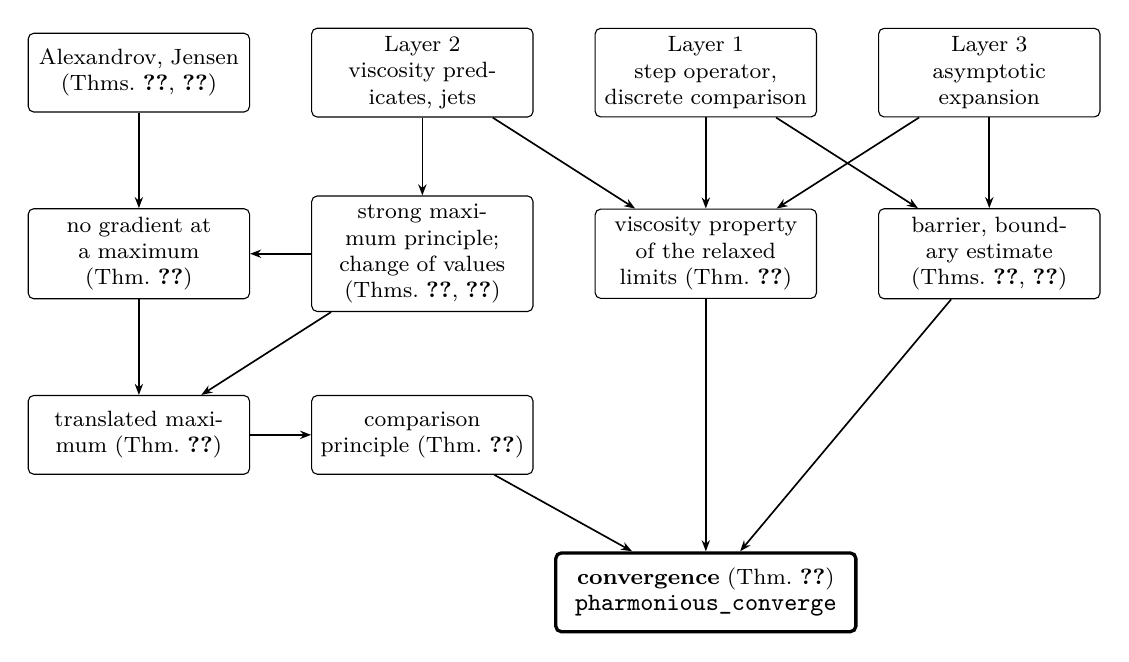
\begin{tikzpicture}[
  box/.style={draw, rounded corners=2pt, align=center, font=\footnotesize,
              text width=2.6cm, minimum height=1.0cm, inner sep=3pt},
  main/.style={box, very thick, text width=3.6cm},
  arr/.style={-{Stealth[length=4pt]}, semithick}]
  % foundations
  \node[box] (AJ) at (0,0)    {Alexandrov, Jensen\\
        (Thms.~\ref{thm:alexandrov}, \ref{thm:jensen})};
  \node[box] (L2) at (3.6,0)  {Layer 2\\ viscosity predicates, jets};
  \node[box] (L1) at (7.2,0)  {Layer 1\\ step operator, discrete comparison};
  \node[box] (L3) at (10.8,0) {Layer 3\\ asymptotic expansion};
  % second row
  \node[box] (S2) at (0,-2.3)   {no gradient at a maximum
        (Thm.~\ref{thm:step2})};
  \node[box] (SC) at (3.6,-2.3) {strong maximum principle; change of values
        (Thms.~\ref{thm:smp}, \ref{thm:cv})};
  \node[box] (V4) at (7.2,-2.3) {viscosity property of the relaxed limits
        (Thm.~\ref{thm:main4})};
  \node[box] (BD) at (10.8,-2.3) {barrier, boundary estimate
        (Thms.~\ref{thm:barrier}, \ref{thm:bdry})};
  % third row
  \node[box] (S3) at (0,-4.6)   {translated maximum
        (Thm.~\ref{thm:step3})};
  \node[box] (CP) at (3.6,-4.6) {comparison principle
        (Thm.~\ref{thm:viscomp})};
  % the theorem
  \node[main] (MT) at (7.2,-6.6) {\textbf{convergence}
        (Thm.~\ref{thm:main})\\ \LEANREF{pharmonious\_converge}};
  % edges
  \draw[arr] (AJ) -- (S2);
  \draw[arr] (L2) -- (SC);
  \draw[arr] (L2) -- (V4);
  \draw[arr] (L1) -- (V4);
  \draw[arr] (L3) -- (V4);
  \draw[arr] (L1) -- (BD);
  \draw[arr] (L3) -- (BD);
  \draw[arr] (SC) -- (S2);
  \draw[arr] (S2) -- (S3);
  \draw[arr] (SC) -- (S3);
  \draw[arr] (S3) -- (CP);
  \draw[arr] (CP) -- (MT);
  \draw[arr] (V4) -- (MT);
  \draw[arr] (BD) -- (MT);
\end{tikzpicture}
\caption{The proof chain of Theorem~\ref{thm:main}. An arrow means that the
target uses the source.}\label{fig:chain}
\end{figure}

\subsection{Working without quotients}\label{ssec:noquot}

Everything operates on concrete function types carrying the predicate of
Definition~\ref{def:bddmeas}, never on Mathlib's quotient $L^p$ spaces.
\cite{AK26} report that moving between concrete functions and $L^p$ elements
forces Lean to resolve long instance chains that can exceed its resource
budget, and they built a bare-function toolkit to avoid it. The dynamic
programming route needs no $L^p$ spaces: the only integrals in the development
are set averages of bounded measurable functions over balls, for which concrete
functions suffice. We record this as the absence of the problem in our setting,
not as a measured comparison; the two developments differ in too many other
respects for one to be meaningful.

% ============================================================================
\section{Formalization notes}\label{sec:notes}

\subsection{Where automation helped and where it did not}
\texttt{exact?} is reliable for locating a single library lemma, and found
\LEANREF{ContDiff.differentiable\_deriv\_two},
\LEANREF{setIntegral\_eq\_zero\_iff\_of\_nonneg\_ae} and
\LEANREF{Measure.addHaar\_ball\_center} at moments when we expected gaps.
\texttt{simp} is the right tool where a goal is definitional unfolding plus a
rewrite. \texttt{fun\_prop} discharged every continuity and measurability side
condition we met.

\texttt{nlinarith} failed repeatedly on goals that were true but required a
specific product it would not invent. In each case computing that product as a
separate hypothesis and switching to \texttt{linarith} succeeded --- for
instance the substitution $\beta M = M - \alpha M$ in
Theorem~\ref{thm:unifarith}, and the collapse
$\alpha M + \beta M = M$ in the rigidity step of
Theorem~\ref{thm:comparison}(ii). The pattern is worth stating: when
\texttt{nlinarith} fails on a goal one believes, supply the missing product
explicitly rather than hoping for a deeper search.

\subsection{Instance requirements invisible informally}
\LEANREF{average\_const} requires \LEANREF{IsFiniteMeasure} and
\LEANREF{NeZero} on the restricted measure. Neither holds automatically for
$\mathrm{volume}|_{B_\eps(x)}$, and \LEANREF{NeZero} genuinely requires
$\eps>0$, so it cannot be a global instance. These had to be supplied as
lemmas before any average manipulation was possible, and every later proof in
that file depends on them.

\subsection{Truncated subtraction}
The exponent $d-1$ produced by \LEANREF{integral\_fun\_norm\_addHaar} is
natural-number subtraction, hence $0$ when $d=0$. Combining
$r^{d-1}\cdot r^2 = r^{d+1}$ therefore requires $0<d$ and is proved by
\texttt{omega}, not \texttt{ring} --- a small point that would silently produce
a wrong constant if the dimension hypothesis were dropped.

\subsection{Shadowing}
Two shadowing incidents each cost several iterations. \texttt{open Filter}
brings a \texttt{min} into scope that shadows the real-number one, producing
errors that point everywhere except the cause. And naming the binary stability
theorem \LEANREF{IsViscositySubsolution.max} makes bare \texttt{max} resolve to
it inside the namespace. Both are avoidable by qualifying or by narrower
\texttt{open} statements.

\subsection{Two abbreviations for one type, deliberately}
\texttt{Average} introduces \LEANREF{EuclSpace} and \texttt{BallMoments}
independently introduces \LEANREF{EuclSpaceM}, both unfolding to
\LEANREF{EuclideanSpace ℝ (Fin d)}. They are definitionally equal, so proofs
compose across the boundary, and the duplication reads at first as an
oversight.

It is not. \texttt{BallMoments} does not import \texttt{Average}, and the
second abbreviation is what allows it to stand alone. We attempted the
unification and it fails immediately: every occurrence of the type becomes an
unknown identifier, because the name it would share lives in a file that is
not a dependency. Repairing that would mean adding the import and coupling two
files that are currently independent.

The independence is worth more than the consistency. The moment computations
are the part of this development most likely to be useful elsewhere, and they
are self-contained precisely because they do not reach into the rest of it.
The same reasoning applies to the \texttt{Diagonal} namespace sitting at the
root rather than inside \texttt{PLaplacian}: it costs an occasional
\LEANREF{\_root\_} qualification and buys the same independence.

We record this because the opposite conclusion is the natural one to draw from
reading the files, and because both of our attempts to tidy these away broke
a working build.

\begin{finding}[Building a chain from both ends produces undischargeable
hypotheses]\label{find:chain}
The characteristic failure is a statement that typechecks, reads correctly, and
has a hypothesis nothing in the development can supply.
\end{finding}

The convergence argument was built from both ends: the discrete side from the
dynamic programming principle forwards, the viscosity side from the predicate
backwards. Five times a statement was proved, committed, and then found to be
unusable or insufficient where it was consumed.

\emph{First.} The limit argument was stated with an \emph{eventual} bound,
\LEANREF{nonneg\_of\_rate}. But the contact points arrive only
\emph{frequently} along the filter: a solution is bounded and Borel, not
continuous (Finding~\ref{find:reg}), so its difference with a test
function need not attain a maximum, and only near-maximizers are available.
Frequently is strictly weaker than eventually, so the two ends did not meet.
The repair is \LEANREF{nonneg\_of\_frequently}, whose proof is four lines: were
the quantity negative, the quotient would eventually exceed it, contradicting
the frequency.

\emph{Second.} Restated with the frequency, the hypothesis asked for a bound on
a function of the parameter alone. But the differential inequality holds at a
near-contact point, where the parameter and the point are coupled; the quantity
bounded depends on both, and the point is not determined by the parameter. No
function of the parameter alone expresses it. The repair is to state the
argument for an arbitrary filter --- its proof never needed otherwise --- and
run it on the product filter where the contact points live
(\LEANREF{nonneg\_of\_frequently'}).

\emph{Third, and earlier.} Two statements of the form ``there exists $K$ with
$\abs{E} \le K\eps^2$'' were written and withdrawn, being provable for any $E$
by taking $K = \abs{E}/\eps^2$ (Finding~\ref{find:vacuous}).

\emph{Fourth.} The upper bound on the supremum of Layer~3 returned some point
with a bound, but did not say that the point was the maximizer; the
localization needs exactly that, at the same point. The repair obtains the
maximizer once and derives every needed property at it
(\LEANREF{sup\_upper\_at\_max}).

\emph{Fifth.} The uniform expansion (Theorem~\ref{thm:expunif}) first exported
its constants without their nonnegativity, which the next step needed. The
repair enlarges each constant to its positive part inside the proof and exports
the sign.

The first two belong to a route later superseded (\S\ref{sec:arch}); the last
two were caught before anything was built on them. All five compiled. All five
read as the intended statement. None was usable as it stood.
What they have in common is that the error lay in a \emph{statement} rather
than a proof, and that it surfaced only on attempting to connect the statement
to what feeds it --- never on reading it back, and never from the elaborator,
which has no notion of whether a hypothesis is satisfiable.

The practical lesson is narrow and we state it as such: when assembling a long
chain, prove the junctions before the segments. A segment whose interface is
wrong is worse than a missing segment, because it looks like progress. The
guard that worked was taking the delicate hypothesis explicitly, as in
Theorem~\ref{thm:opbounded}, so that the interface is visible in the statement
and a mismatch is a type error rather than a dead end.

\begin{finding}[Irregularity is paid for in quantifiers]\label{find:quant}
The discrete solution's lack of continuity reaches three separate points of the
convergence argument, and at each it costs an extra quantifier rather than a
different proof.
\end{finding}

A $p$-harmonious function is bounded and Borel but not continuous
(Finding~\ref{find:reg}), so the difference $u_\eps - \varphi$ need not attain
a maximum on a closed ball and only near-maximizers are available. We had
expected this to be the principal difficulty of the convergence layer. It
appears three times, and each time the remedy is to weaken a quantifier.

\emph{In the limit argument.} The contact points arrive \emph{frequently} along
the filter, not eventually, so the limit argument as first proved did not
apply. In the first route the repair was a frequent form of the limit argument
(\LEANREF{nonneg\_of\_frequently}). In the final proof no limit is taken at
all: the argument is by contradiction, and needs only one parameter at which
the frequent condition and finitely many eventual ones hold together.

\emph{In the comparison.} The comparison through the operator wants the
difference to equal its bound; the near-contact gives it only within $\kappa$.
The repair carries $\kappa$ into the conclusion
(\LEANREF{dpp\_comparison\_approx}): the inequality becomes
$\varphi(y) \le \Op\varphi(y) + \kappa$, and the slack passes through the
expansion as an additive term. An earlier version of this document said that the
slack then vanishes in the limit, $\kappa$ being arbitrary. That is false.
Isolating the operator divides by $\eps^2$, so $\kappa$ must shrink faster than
$\eps^2$, and it can be tied to $\eps$ only when the near-maximizer is measured
against the parameter's own supremum (Finding~\ref{find:refpoint}); with
$\kappa = \eps^3$ the term is of order $\eps$.

\emph{In the ball containment.} The local maximum bounds the difference on a
ball about the base point; the comparison needs it on a ball about the
near-contact point. The repair is the triangle inequality with both the
parameter and the displacement below half the radius
(\LEANREF{ball\_subset\_of\_near}), conditions which hold eventually along the
filter, so their intersection with a frequency is still a frequency.

What the three have in common is that no new analysis was required at any of
them: the mathematical content is unchanged and only the logical form of the
statements had to be adjusted. We record it because the opposite expectation
--- that a regularity failure must be met with a regularity argument --- is the
natural one, and because locating where irregularity bites is cheaper than
strengthening the hypotheses to avoid it.

\subsection{What we would do differently}

Settle the open-versus-closed ball question from the literature before writing
any operator code, since it is a hypothesis of the whole development rather
than a detail (Finding~\ref{find:closedball}). Read the uniqueness proof before
building infrastructure aimed at it: Finding~\ref{find:mpr} invalidated
\S\ref{ssec:psi} as a route, and Finding~\ref{find:notadd} would have shown the
same from the operator's algebra alone. Narrow imports from the start; one file
went from six minutes to eighty seconds when a single unnecessary import was
removed. For the convergence layer, write down every uniformity the argument
needs before proving any of it (Finding~\ref{find:locunif}), and prove the
junctions between results before the results themselves
(Finding~\ref{find:chain}): roughly a third of the layer's lines belong to a
route assembled around interfaces that did not meet. And distrust estimates of
the work remaining in an assembly. Each junction surprise added files that no
estimate had foreseen, and it was the step most often deferred --- here,
dividing by $\eps^2$ --- that held the gap.

% ============================================================================
\section{Future work}\label{sec:future}

\subsection{Stability for the \texorpdfstring{$\eps$}{epsilon}-problem}

Theorem~\ref{thm:discunique} gives uniqueness for equal data. The stability
estimate $\sup_\Omega\abs{u' - u} \le \sup_{\Gamma_\eps}\abs{g' - g}$ of
\cite[Theorem~2.2]{LPS14}, for solutions with data $g$ and $g'$ on the strip,
would follow from the same propagation argument, with the bound for $w$ outside
$\Omega$ replaced by $\sup_{\Gamma_\eps}(g' - g)$.

\subsection{Contributions to Mathlib}

Alexandrov's theorem, Jensen's lemma, the strong maximum principle for the
normalized $p$-Laplacian, and the uniqueness of Peano expansions are of
independent value, and the first two at least are natural candidates for
Mathlib.

\subsection{The infinite stability theorem}

For an infinite family of subsolutions the supremum need not be upper
semicontinuous, so one passes to the envelope, and then a contact point for the
envelope is not a contact point for any single member. The argument that
handles this is, in structure, the one of \S\ref{ssec:nearmax}: near-maximizers,
measured against each member's own supremum, converging to the point of contact
by strictness. Much of Layer~4 should therefore transfer.

\subsection{Longer term}

In increasing order of difficulty: the game layer proper --- strategies,
trajectory measures via \LEANREF{ProbabilityTheory.Kernel}, exit times as
\LEANREF{IsStoppingTime}, and identification with the game value via optional
stopping, recovering \cite[Thm.~3.2]{LPS14}; the case $1 < p < 2$, through the
regrouped operator; variable coefficients, obstacle problems and Neumann
conditions; and the parabolic case, which \cite[\S5]{LPS14} note is
considerably easier than the elliptic one.

\subsection{How the development was produced}

As in \cite{AK26}, the formalization was carried out with extensive use of a
large language model, Anthropic's Claude, in conversation. The mathematical
route came from the authors and the literature: the layer structure, the
analytic rather than probabilistic existence proof, and the comparison argument
of \S\ref{sec:comparison}. The model proposed formal statements and drafted Lean
files, one file or one lemma at a time. Every draft was compiled by the second
author on the pinned toolchain, and the compiler's output was returned
verbatim, so that each correction was driven by an error message rather than
by the model's own assessment of its draft. Statements were fixed before proofs
(Finding~\ref{find:junctions}). No trust is placed in the model beyond what is
placed in any author of a draft: the artifact is checked by Lean's kernel, and
the main theorem depends only on the standard axioms. Several findings of
\S\ref{sec:findings}, among them the closed-ball defect and the restriction to
$p \ge 2$, surfaced as drafts that typechecked but whose proofs would not go
through.

% ============================================================================
\section*{Acknowledgements}
We thank the Mathlib community, on whose library this development is built,
and the developers of Lean. This work received no external funding.

% ============================================================================
\bibliographystyle{amsplain}
\bibliography{refs}

\end{document}
